
\documentclass[bachelor,print,msfonts]{xduthesis}
%\documentclass[bachelor,print]{xduthesis}

\usepackage{listings}
\usepackage{overpic}
\usepackage{algorithm}
\usepackage{algorithmicx}
\usepackage{algpseudocode}
\usepackage{booktabs}
\usepackage{colortbl}
\usepackage{multirow}
\usepackage{pgfplots}
\usepackage{mathtools}
\newtagform{EueTag}{式~(}{)}
\usetagform{EueTag}
\lstset{language=TeX, basicstyle=\ttfamily}

\newcommand{\figref}[1]{图\ref{#1}}
\newcommand{\sArt}{state-of-the-art}
\newcommand{\wyh}[1]{{\textcolor{blue}{#1}}}
\newcommand{\secref}[1]{Sec. \ref{#1}}
\newcommand{\tabref}[1]{Tab.~\ref{#1}}
\newcommand{\thudot}[1]{}
\renewcommand{\emph}[1]{\texttt{#1}}

\floatname{algorithm}{算法}
\renewcommand{\algorithmicrequire}{\textbf{输入:}}
\renewcommand{\algorithmicensure}{\textbf{输出:}}

\newcommand{\mypara}[1]{\paragraph{#1.}}

\begin{document}

%%%%%%%%%%%%%%%
%% 论文前置部分
%%%%%%%%%%%%%%%
\frontmatter

% 论文相关信息(封面)
\classid{1513018}
\studentid{15130188018}

\cschool{计算机科学与技术学院}
\ctitle{基于多任务学习的文本\\表示方法研究}
\cauthor{孙天祥}
\cmajor{软件工程}
\csupervisor{刘西洋~教授}

% 中英文摘要声明
\begin{cabstract}
	文本表示是自然语言处理的必要任务,表示方法的好坏对于模型性能起着至关重要的作用。为得到泛化能力强的文本表示,近年来多任务学习被广泛应用在各大自然语言处理任务中,通过联合学习多个相关任务来共享任务间的知识,从而提升模型在各个任务上的表现。
	
	近年来,一种新型的神经网络模型Transformer因其在机器翻译和迁移学习等方面取得的巨大成功开始在自然语言处理领域流行。然而,之前的工作大都在卷积网络和循环网络上研究多任务学习的共享结构,目前还很少有工作探究Transformer上的多任务共享架构。本文在Transformer上探索了句子级的多任务文本表示方法:首先设计了两种传统的硬共享结构,接着提出了两种逐层共享结构,能够在每一层根据输入动态地抽取其他任务的特征来形成任务特定表示。我们在16个情感分析任务上进行了实验,对比单任务模型,四种多任务模型的准确率均取得了较大提升,其中,本文提出的两种逐层共享结构均超越了传统共享结构。实例可视化分析的结果解释了模型的有效性,并展示了任务之间的相关性。
	
	最后,总结了本文工作与已有研究的异同,概括了本文的创新性与局限性,并展望了未来多任务学习在自然语言处理领域的发展前景。
\end{cabstract}


\begin{ckeywords}
	自然语言处理\ \ \ \ \ \ 多任务学习\ \ \ \ \ \ Transformer\ \ \ \ \ \ 表示学习
\end{ckeywords}

%\cthesistype{应用基础技术}


\begin{eabstract}
	Language representation is an essential task for natural language processing(NLP). Representation method plays a crucial role in the performance of the model. To obtain a general representation, multi-task learning(MTL) methods, which allow models to share knowledge between related tasks, are widely applied to many NLP tasks.
	
	Recently, Transformer, a novel neural network based on self-attention mechanism, has become popular in the field of NLP due to its great success in machine translation and transfer learning. However, most of the previous work has focused on designing multi-task sharing scheme for convolutional networks and recurrent networks. There is little exploration on multi-task learning in Transformer. In this paper, we propose 4 sentence-level multi-task transformer architectures: two traditional hard sharing architectures and two layerwise sharing architectures, which can dynamically extract features of related tasks and form task-specific representation based on the input at each layer. We conduct experiments on 16 sentiment analysis tasks. Our 4 multi-task transformers consistently outperform transformers trained with single task. Besides, the proposed layerwise sharing architectures achieve better accuracy than traditional architectures. Case study and visualization explain the validity of the proposed models and demonstrate the relationship between tasks.
	
	Finally, we summarize the similarities and differences between our proposed models and existing work, point out our contributions and defects.
	
\end{eabstract}


\begin{ekeywords}
	Natural Language Processing\ \ \ \ Multi-Task Learning\ \ \ \ Transformer\ \ \ \ Representation Learning
\end{ekeywords}

%\ethesistype{Applied Basic Technology}

% 生成论文的封面、声明页、中英文摘要
\makecover
\tocmatter

% 论文目录
\tableofcontents

%%%%%%%%%%%%%%%
%% 论文正文
%%%%%%%%%%%%%%%
\mainmatter

\chapter{绪论}
\label{cha:intro}
本章首先介绍基于深度学习的自然语言处理的研究背景,阐述在该背景下多任务学习的研究价值及意义。接着简要介绍自然语言处理和多任务学习的研究进展,并指出目前存在的问题。然后介绍本文的研究内容及目标,并概括了本文工作的创新之处。本章的最后给出了论文的主要内容和章节安排。

\section{研究背景及意义}
1950年,阿兰·图灵(Alan Turing)提出了著名的\emph{图灵测试}\footnote{图灵测试是指,一个人在不接触对方的情况下,通过某种方式和对方进行一系列的问答。若在相当长时间内,他无法根据问答的情况判断对方是人还是机器,那么可以认为该机器具备智能。},直接推动了人工智能从哲学探讨的层面上升到科学研究。随后不久,在1956年举办的达特茅斯会议上,\emph{人工智能}(Artificial Intelligence,AI)的概念被正式提出,John McCarthy将这一新兴领域的研究目标定义为:“让机器的行为看起来像人类所表现出来的智能行为一样”。自1956年至今的六十余年中,研究人员尝试了多种方法来实现这一愿景,人工智能领域也随着这些方法的成功与失败经历了数次热潮与低谷。近年来,随着数据量的增加和算力的增强,以神经网络为代表的\emph{深度学习}(Deep Learning)异军突起,在语音识别\cite{DBLP:conf/asru/MikolovDPBC11}\cite{DBLP:conf/apsipa/LiHYW13}、计算机视觉\cite{DBLP:journals/cacm/KrizhevskySH17}\cite{DBLP:journals/pami/FarabetCNL13}\cite{DBLP:conf/nips/TompsonJLB14}等众多应用场景中取得了巨大突破,再次掀起了人工智能的研究热潮。

\emph{自然语言处理}(Natural Language Processing, NLP)被很多人认为是“人工智能皇冠上的明珠”,致力于使计算机具备理解和生成人类语言的能力。随着深度学习技术的发展,越来越多的研究者开始使用深度学习的技术解决自然语言处理中的难题\cite{DBLP:journals/jmlr/CollobertWBKKK11}\cite{DBLP:conf/emnlp/BordesCW14}\cite{DBLP:conf/acl/JeanCMB15}\cite{DBLP:conf/nips/SutskeverVL14},在很多任务上远远超越了之前的传统方法。

然而,像绝大多数领域一样,对NLP领域的研究常常被划分为多个任务,如命名实体识别、阅读理解、机器翻译等。目前一般的做法是为当前关注的某一个任务设计特定的神经网络模型,在此单一任务及数据集上进行训练。遗憾的是,这样设计出来的模型常常具有较大的局限性,在某个数据集上表现优秀的模型可能在另一个数据集上就会表现很差,即使这两个数据集来自同一任务。并且,由于NLP任务及数据集众多,一时之间各种神经网络结构层出不穷。深度学习刚刚帮助人们从“特征工程”中脱离出来,很快又陷入了所谓的网络“结构工程”。同时,这也将模型限制在了特定领域,难以发展出更为通用的智能系统。

为解决这一问题,很多研究人员转而寻求泛化能力更加强大、能够提取数据更一般性的特征表示的模型,而不是为每一个新的任务甚至数据集设计新的模型。很快,人们发现通过迁移学习和多任务学习能够得到这样的模型。在计算机视觉领域,在ImageNet\cite{DBLP:conf/cvpr/DengDSLL009}这样的大规模图像分类数据集上预训练的模型能够在很多图像分类任务上表现良好;在NLP领域,通过在大规模无标注文本上预训练一个语言模型也通常能够给各种下游任务带来很大收益\cite{DBLP:conf/naacl/PetersNIGCLZ18}\cite{radford2018improving}。这些发现表明,共享模型在其他任务上学习到的知识能够显著提升模型的性能,而且通常比改进网络结构所带来的收益更大。

在这一背景下,人们开始思考:\textbf{是否可以训练单个模型来处理几乎所有的NLP任务?}近年来,多任务学习被广泛地应用在深层神经网络中,在序列标注、文本分类、机器翻译等多个经典NLP任务上都取得了令人鼓舞的效果。随着多任务学习的引入,人们发现很多NLP任务可以归纳为统一的模型范式,如问答范式\cite{mccann2018natural}、分类范式\cite{radford2018improving}\cite{devlin2018bert}。同时,越来越多的研究者开始关注模型在多任务上的表现,出现了decaNLP\cite{mccann2018natural}、GLUE\cite{DBLP:conf/emnlp/WangSMHLB18}等大规模多任务评测数据集。可以预见,在预训练模型已经取得了巨大成功的基础上,随着多任务学习算法的成熟以及多任务评测基准的规范化,通用神经网络模型还将给自然语言处理领域乃至整个人工智能领域带来更多的惊喜。

\section{相关研究进展}

本节将简要介绍深度学习背景下的自然语言处理、多任务学习、迁移学习以及它们相结合的研究进展及现状,并阐述了它们之间的联系以及目前存在的不足。

自然语言处理(Natural Language Processing, NLP)是一门旨在使得计算机具备处理、理解和生成自然语言(人类语言)能力的学科。近年来,以神经网络为代表的深度学习在自然语言处理\cite{DBLP:journals/jmlr/CollobertWBKKK11}\cite{DBLP:conf/emnlp/BordesCW14}\cite{DBLP:conf/acl/JeanCMB15}\cite{DBLP:conf/nips/SutskeverVL14}中取得了广泛的成功。然而,不同于语音、图像等连续实值信号,自然语言是由离散的符号构成,这使其难以直接作为神经网络的输入。为解决这一问题,人们使用低维稠密向量来表征文本的语义信息\cite{DBLP:conf/nips/MikolovSCCD13}\cite{DBLP:conf/emnlp/PenningtonSM14},由于语义信息被分布到向量的各个维度,因此这种方法被称为分布式表示。随着分布式表示的引入,深度学习在自然语言处理领域得到了广泛的应用,卷积神经网络(Convolutional Neural Network, CNN)、循环神经网络(Recurrent Neural Network, RNN)相继被用于处理文本数据,近年来又提出了完全基于自注意力机制的全连接网络Transformer。这些神经网络的应用使得过去很多难以解决的NLP问题上取得了巨大进展。

事实上,文本的分布式表示的好坏对于模型的性能起着至关重要的作用。以分类任务为例,给定数据的一个好的表示,即使简单的线性分类器也能取得非常高的分类准确率\cite{tenney2018you}\cite{liu2019linguistic}。进入深度学习时代以来,自然语言处理领域中取得的许多突破都来自于对文本的通用表示方法的研究,如word2vec\cite{DBLP:conf/nips/MikolovSCCD13},ELMo\cite{DBLP:conf/naacl/PetersNIGCLZ18},BERT\cite{devlin2018bert}等。然而,相较于语音和图像数据,由于文本数据本身的离散性和歧义性,以及标注成本高、难度大等问题,如何得到一个好的文本表示仍然是自然语言处理领域的重大难题。

从机器学习的角度来看,一个好的表示方法除了能够在对应任务上表现良好,还应当具备良好的可迁移性与泛化能力,即能够在相似任务和新数据上获得较好的效果。在自然语言处理领域,常常使用\emph{多任务学习}(Multi-Task Learning, MTL)和\emph{迁移学习}(Transfer Learning)的方法来得到这样的文本表示\cite{devlin2018bert}\cite{DBLP:conf/icml/CollobertW08}。

多任务学习可以追溯到1993年\cite{DBLP:conf/icml/Caruana93},它是指同时使用多个任务对模型进行训练,使其学习到数据的某种泛化表示,该表示能够同时解释这多个任务。在过去的几年里,大量研究人员探索了多任务学习在卷积神经网络和循环神经网络上的应用模式,验证了基于神经网络的多任务学习在文本表示上的有效性。Collobert等人\cite{DBLP:conf/icml/CollobertW08}使用一个简单的卷积网络来同时学习词性标注、语块标注、命名实体识别、语义角色标注、语义相似度和语言模型等多个任务,超越了使用单任务训练的效果。随着循环神经网络在NLP上的广泛应用,研究者开始基于循环网络构造多任务学习框架,在机器翻译\cite{DBLP:conf/acl/DongWHYW15}、文本分类\cite{DBLP:conf/ijcai/LiuQH16}\cite{DBLP:conf/acl/LiuQH17}、序列标注\cite{DBLP:conf/acl/SogaardG16}等常见NLP任务上均取得了成功。多任务学习的一个关键问题在于如何设计一个高效的共享模式来允许模型共享多个任务的知识。上述提到的工作也大都致力于为所要解决的问题以及采用的网络结构来设计合适的共享模式。

同时,也有大量工作致力于使用迁移学习的范式来获取文本的通用表示,一般做法是利用语言模型\cite{DBLP:conf/naacl/PetersNIGCLZ18}\cite{radford2018improving}、机器翻译\cite{DBLP:conf/nips/McCannBXS17}以及其他无监督任务\cite{devlin2018bert}来预训练一个可迁移的模型。并且,迁移学习与多任务学习本身并不互斥,因此可以同时利用二者的方法,使用多任务预训练迁移模型\cite{DBLP:conf/iclr/SubramanianTBP18},也可以在预训练得到的模型的基础上再使用多任务来微调\cite{liu2019multi}\cite{anonymous2018bam!}。

事实上,多任务学习和迁移学习本质上都是通过共享参数来迁移模型在不同任务中学习到的知识,并以此来提升泛化能力。因此,通常在迁移学习中效果很好的模型也可以应用在多任务学习中。近期,以Transformer为预训练网络结构得到的迁移模型GPT\cite{radford2018improving}和BERT\cite{devlin2018bert}在诸多自然语言处理任务上取得了极大的提升,这证明了Transformer强大的文本表示能力。然而,不同于CNN和RNN,目前还很少有工作研究多任务学习在Transformer上的应用模式,已有的少量工作也只是将最传统的多任务共享模式简单地应用在Transformer中\cite{liu2019multi}。

\section{本文研究内容}

本文试图在一定程度上填补目前多任务学习在Transformer结构下的研究空缺。首先,本文较为系统地考察了传统多任务学习架构在Transformer上的应用效果,然后,根据Transformer自身的结构特点设计了新的多任务学习架构。

在CNN及RNN结构中应用多任务学习通常是“纵向”的,即在网络结构的某一层上堆叠任务特定层\cite{DBLP:conf/acl/SogaardG16}\cite{DBLP:conf/ijcai/ZhengCQ18}。这种架构蕴含着一个假设:存在某种通用的文本表示,特定的任务表示可以由该通用表示通过简单的变换得到。然而,这样的假设限制了能够同时学习的任务的多样性,难以处理弱相关任务及不同难度的任务。有一些工作采用了“横向”共享的架构,即允许模型使用其他任务的模型在同一层的隐状态\cite{DBLP:conf/ijcai/LiuQH16}\cite{DBLP:conf/cvpr/MisraSGH16}\cite{1705.08142},然而这些架构也存在两个问题:(1)通常需要为每个任务训练一个模型,参数量大且难以扩展;(2)各任务模型之间的信息交互难以控制。

而在Transformer中,可以很容易地在“横向”以记号的形式进行扩展,并且扩展的记号可以像普通单词一样与句子中的每个单词进行交互,只需增加少量参数。基于这一特性,本文给出了两种新型多任务共享模式:层级-隐式共享模式和层级-显式共享模式,并通过大量实验证明了两种模式的有效性。

\section{论文结构}

本文主要内容包括介绍已有的基于多任务学习的文本表示方法,几种新型的多任务文本表示模型及其实验结果,工作总结及对未来的展望。全文分为五个章节进行介绍,具体结构安排如下:

第~\ref{cha:intro}~章,介绍研究背景及意义,概括本文的研究内容。

第~\ref{cha:related_work}~章,介绍相关的理论基础及前沿进展。在~\ref{sec:dl}~节介绍深度学习的相关概念;在~\ref{sec:mtl}~节介绍基于神经网络的多任务学习;在~\ref{sec:nlp}~节介绍深度学习背景下自然语言处理的发展现状;在~\ref{sec:mtl4nlp}~节介绍多任务学习在自然语言处理中的应用。

第~\ref{cha:model}~章,详细介绍本文研究的模型结构及实现细节。在~\ref{sec:tf}~节介绍Transformer的模型结构;在~\ref{sec:mtl_tf}~节介绍几种多任务Transformer架构;在~\ref{sec:imp}~节给出本文所使用的超参数设置以及实现细节。

第~\ref{cha:exp}~章,介绍实验相关的信息。在~\ref{sec:task}~节描述模型应用的具体任务;在~\ref{sec:ds}~节给出本文使用的各个数据集的有关信息;在~\ref{sec:results}~节介绍模型在各数据集上的实验结果;最后在~\ref{sec:analysis}~节对模型进行了实例可视化分析。

第~\ref{cha:conclusions}~章,对本文的贡献和不足进行总结,回顾相关领域面临的机遇与挑战,并给出了未来的研究方向。


\chapter{相关背景与研究进展}
\label{cha:related_work}
本文研究的内容包含了深度学习、多任务学习与自然语言处理三个主题,这里首先阐述这些主题之间的联系,接着分别介绍它们各自的相关概念与研究进展,最后介绍了三者交叉的一些重要研究工作。

我们利用深度学习与多任务学习来解决自然语言处理中的问题,具体的,即在深层神经网络中使用多任务学习来获得文本的泛化表示。从这一角度来看,深度学习与多任务学习是我们的工具,而自然语言处理为我们的应用场景。同时,深度学习与多任务学习都可以归为机器学习问题,而他们二者又有交叉,如图~\ref{fig:ml_dl_mtl}~所示。

\begin{figure}[htb]
	\centering
	\begin{tikzpicture}[scale=0.75]
	\draw (-4,3) rectangle (4,-3);
	\draw[draw = black] (-1.5,0) circle (2);
	\draw[draw = black] (1.5,0) circle (2);
	\node at (-2.8,2.5) {机器学习};
	\node at (-2,0) {深度学习};
	\node at (2,0) {多任务学习};
	\end{tikzpicture}
	\caption{机器学习、深度学习、多任务学习的关系}
	\label{fig:ml_dl_mtl}
\end{figure}

\section{深度学习与神经网络}
\label{sec:dl}
近年来,\emph{深度学习}(Deep Learning)发展十分迅速,在人工智能的很多子领域上取得了巨大成功,如语音识别\cite{DBLP:conf/asru/MikolovDPBC11}\cite{DBLP:conf/apsipa/LiHYW13}、计算机视觉\cite{DBLP:journals/cacm/KrizhevskySH17}\cite{DBLP:journals/pami/FarabetCNL13}\cite{DBLP:conf/nips/TompsonJLB14}、自然语言处理\cite{DBLP:journals/jmlr/CollobertWBKKK11}\cite{DBLP:conf/emnlp/BordesCW14}\cite{DBLP:conf/acl/JeanCMB15}\cite{DBLP:conf/nips/SutskeverVL14}等。

从要研究的问题来看,深度学习属于机器学习的一个分支,都是研究如何从有限个样例中通过某种算法总结出一般性规律或模式,并将其应用到新的未知数据上去。例如,通过机器学习或深度学习算法,可以根据历史病例总结出症状与疾病之间的规律,当遇到新的病人时可以利用算法总结出来的规律来帮助判断这个病人得了什么疾病\footnote{例子来源:《神经网络与深度学习》,邱锡鹏,\url{https://nndl.github.io}}。

同时,深度学习又与机器学习有很大的不同。从模型的构成来说,深度学习模型一般更加复杂,参数量更多。由于数据从输入到输出需要经过多个线性或非线性组件,信息传递路径较长,因此被称作深度学习。深度学习模型的一个最典型代表就是\emph{人工神经网络}(Artificial Neural Network,ANN),下面简称\emph{神经网络}。神经网络是一种受人脑神经系统启发的复杂数学模型,由神经元以及它们之间的连接组成。通过这些神经元的加工,原始数据从底层特征开始经过一道道加工逐渐转换为抽象的高层语义特征。

总的来说,神经网络可以被看做一个包含大量参数的复合函数,该函数描述了输入和输出之间的复杂关系,因此可以被用于处理很多模式识别任务,如语音识别、图像识别等。形式化地,神经网络可以这样描述:
\begin{equation}
	y = \mathcal{F}(\mathbf{x} \mid \theta).
\end{equation}
其中,函数~$\mathcal{F}$~受参数~$\theta$~控制。

给定包含大量样例的集合,参数~$\theta$~可以通过随机梯度下降等优化算法得到,求解参数的优化过程就被称为\emph{学习过程},通过学习得到的参数被称为\emph{可学习参数},常简称为\emph{参数}。还有一部分不可以被学习的参数,例如神经网络的层数,被称为\emph{超参数},意为控制参数的参数,超参数通常根据经验指定或根据实验效果来确定。

前面提到,参数学习需要一个包含大量样例的集合,该集合就是\emph{数据集}。在有监督学习中,每个样例一般包含输入~$\mathbf{x}$~和输出~$y$,输出也常被称为标签。其中,输入一般为一个向量,向量的每一个维度表示了样本的一个属性;输出一般为一个标量。包含~$n$~个样例的集合~$\mathcal{D} = \{ \mathbf{x}_i, y_i \}_{i=1}^n$~就是数据集。在实际使用时,数据集通常被划分为训练集、验证集(也叫开发集)和测试集。其中,用训练集来让算法学习参数,用验证集来调整算法的超参数,用测试集来衡量模型的优劣。

给定数据集~$\mathcal{D}$~和模型结构,即~$\mathcal{F}$的形式,优化算法可以得到参数~$\theta$~进而确定模型~$\mathcal{F}(\theta)$. 下面介绍一种简单的前馈神经网络结构:\emph{多层感知机}(Multi-Layer Perceptron, MLP)。一个单隐层的MLP可以记作~$\mathcal{F}(\mathbf{x}; \theta) = \mathbf{w}_2(f(\mathbf{w}_1\mathbf{x} + b_1))+b_2$,其中参数~$\theta = \{ \mathbf{w}_1, b_1, \mathbf{w}_2, b_2 \}$,函数~$f(\cdot)$~为非线性激活函数,如ReLU. 多层感知机的结构如图~\ref{fig:mlp}~所示,为简单起见,图中省略了偏置项~$b_1, b_2$.

\begin{figure}[htb]
	\def\layersep{2.5cm}
	\centering
	\begin{tikzpicture}[shorten >=1pt,->,draw=black!50, node distance=\layersep]
	\tikzstyle{every pin edge}=[<-,shorten <=1pt]
	\tikzstyle{neuron}=[circle,fill=black!25,minimum size=17pt,inner sep=0pt]
	\tikzstyle{input neuron}=[neuron, fill=white!50, draw=black];
	\tikzstyle{output neuron}=[neuron, fill=white!50, draw=black];
	\tikzstyle{hidden neuron}=[neuron, fill=lightgray!50, draw=black];
	\tikzstyle{annot} = [text width=4em, text centered]
	
	% Draw the input layer nodes
	\foreach \name / \y in {1,...,4}
	% This is the same as writing \foreach \name / \y in {1/1,2/2,3/3,4/4}
	\node[input neuron, pin=left:$x_{\y}$] (I-\name) at (0,-\y) {};
	
	% Draw the hidden layer nodes
	\foreach \name / \y in {1,...,5}
	\path[yshift=0.5cm]
	node[hidden neuron] (H-\name) at (\layersep,-\y cm) {};
	
	% Draw the output layer node
	\node[output neuron,pin={[pin edge={->}]right:$y$}, right of=H-3] (O) {};
	
	% Connect every node in the input layer with every node in the
	% hidden layer.
	\foreach \source in {1,...,4}
	\foreach \dest in {1,...,5}
	\path (I-\source) edge (H-\dest);
	
	% Connect every node in the hidden layer with the output layer
	\foreach \source in {1,...,5}
	\path (H-\source) edge (O);
	
	% Annotate the layers
	\node[annot,above of=H-1, node distance=1cm] (hl) {隐藏层};
	\node[annot,left of=hl] {输入层};
	\node[annot,right of=hl] {输出层};
	\end{tikzpicture}
	\caption{多层感知机}
	\label{fig:mlp}
\end{figure}

随着深度学习的发展,神经网络的结构也变得日益多样和复杂。上面的多层感知机属于全连接前馈网络,而前馈网络的另一典型代表就是在计算机视觉中被广泛使用的\emph{卷积神经网络}(Convolutional Neural Network, CNN),它与全连接网络的区别在于权重共享和局部连接。除前馈网络外,还有一类网络称为反馈网络,因为反馈网络的神经元可以接收来自本身的反馈信号,从而具备一定的记忆能力,因此也被称为记忆网络。反馈网络的一种典型代表就是\emph{循环神经网络}(Recurrent Neural Network, RNN),它在自然语言处理中得到了广泛应用。另外,近年来\emph{图神经网络}(Graph Neural Network, GNN)因其在处理图结构数据上的优势也得到了迅速发展,近期也被用于处理文本和图像数据。

深度学习能够成功的重要原因在于其强大的特征表示能力。在传统的机器学习中,通常需要人为地构造数据特征,再训练一个学习算法来总结这些构造出来的特征输入与输出之间的关系。例如,在文本分类任务中,传统机器学习的做法一般是利用词袋模型或TF-IDF来构造文本特征,再将其作为支持向量机等分类器的输入来进行分类。而在深层神经网络中,算法自动学习原始数据的特征表示,数据从输入到输出的过程~$\mathbf{x}\to \mathcal{F} \to y$~可以人为地划分为两个阶段:\emph{表示}和\emph{预测}\footnote{有时也被称为编码和解码}。所谓表示,就是神经网络中间隐层的状态,上文中MLP的中间隐层就可以当作某种浅层表示;而预测,比如分类或回归,一般是在上一层得到的特征表示的基础上进行进一步变换得到易于预测的任务特定表示。因此,深度学习又可以看作是一种表示学习,而深度学习的成功也证明了学到好的特征表示的重要意义。

\section{多任务学习}
\label{sec:mtl}
在机器学习中,我们通常关心模型在某个任务上的某个指标,并通过在某个数据集上训练单个模型或一组集成模型来达成此目标。事实上,有时我们可以同时利用其他数据集甚至其他任务来联合训练模型,从而进一步提升性能,这种方法就是\emph{多任务学习}(Multi-Task Learning, MTL)。

从定义上来说,多任务学习就是一种归纳转移(Inductive Transfer)方法,通过利用包含在相关任务训练信号中的领域特定信息来提升模型的泛化能力\cite{Caruana1997}。在机器学习中,给定训练集,存在多个假设能够解释训练数据,这些假设构成的空间被称为假设空间,假设空间中的一个假设就对应了一个模型。不同的机器学习算法倾向于选择不同的假设,这种选择偏好被称为\emph{归纳偏置}(Inductive Bias)。直观上,多任务学习使得算法倾向于选择一种能够同时解释多个任务的假设,也即引入了多个任务的归纳偏置。从表示学习的角度看,这样能够同时适用于多个任务的表示就是泛化的表示。图~\ref{fig:mtl_int}~较为直观地给出了多任务学习的一种解释。

\begin{figure}[htb]
	\centering
	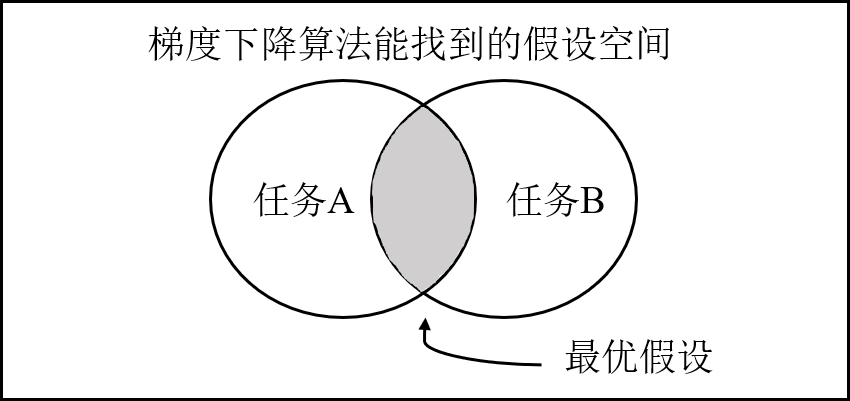
\includegraphics[scale=0.55]{mtl_int.png}
	\caption{多任务学习的一种直观解释}
	\label{fig:mtl_int}
\end{figure}

关于多任务学习为何有效,除了上面的解释(归纳偏置)之外,Caruana还给出了几种合理的解释\cite{Caruana1997}:

\begin{itemize}
	\item \textbf{数据增强(Statistical data amplification)} 由于多个任务的数据集通常是不同的,使用多个相关任务对同一个模型进行训练相当于增大了训练数据量。
	\item \textbf{特征选择(Attribute selection)} 如果任务噪声较大,或者数据高维而数据量有限,模型很难分辨相关特征和无关特征,而多任务学习可以帮助模型选出相关特征,因为这些特征通常在多个任务中是共用的。也就是说,其他任务为模型选择特征提供了额外的证据。
	\item \textbf{窃听(Eavesdropping)} 存在某些特征对于任务 $A$ 易于学习,而对于任务 $B$ 则难以学习。通过多任务学习,模型可以在执行任务 $B$ 时使用任务 $A$ 学到的特征。
\end{itemize}

在深度学习之前,多任务学习已经被应用在线性模型、核方法、决策树、多层感知机等传统机器学习算法上,有大量的研究集中在稀疏正则化\cite{DBLP:conf/nips/ArgyriouEP06}\cite{DBLP:conf/colt/LouniciPTG09}以及学习任务之间的关系\cite{DBLP:journals/jmlr/EvgeniouMP05}\cite{DBLP:conf/nips/JacobBV08}上。

随着深度学习的发展,多任务学习开始应用在深层神经网络中,并在自然语言处理\cite{DBLP:conf/icml/CollobertW08}、计算机视觉\cite{DBLP:conf/cvpr/MisraSGH16}、语音识别\cite{DBLP:conf/icassp/DengHK13}、药物设计\cite{DBLP:journals/corr/RamsundarKRWKP15}等众多应用场景中取得了成功。同时,多任务学习作为一种模型无关的方法,在卷积神经网络\cite{DBLP:conf/icml/CollobertW08}\cite{DBLP:conf/cvpr/MisraSGH16}、循环神经网络\cite{DBLP:conf/ijcai/LiuQH16}、图网络\cite{liu2018multi}上都可以应用。

然而,无论是在传统机器学习算法上还是在深层神经网络上,多任务学习的核心观点都在于知识共享。如何为特定任务和学习算法设计合适的共享模式一直是多任务学习的重要问题。从多任务学习的应用方式来看,可以大概分为下面四种共享模式:

\begin{itemize}
	\item \textbf{硬共享模式}:为多个任务联合训练单个模型,让不同任务共享相同的神经网络层来提取任务无关的通用特征表示,每个任务通过自己的任务特定层在通用表示基础上进行加工得到任务特定表示。
	\item \textbf{软共享模式}:为每个任务训练自己的模型,但每个任务都可以窃听其他任务的模型学习到的特征表示。窃听的方式可以是注意力机制、门控机制,也可以是简单的线性加权。
	\item \textbf{分层共享模式}:为多个任务联合训练单个模型,但简单任务在神经网络低层施加监督信号,困难任务在神经网络的高层施加监督信号。
	\item \textbf{共享-私有模式}:为每个任务训练单个模型,同时使用多个任务训练一个共享模型。每个任务的模型在提取自己任务特定表示的时候也可以从共享模型中提取任务无关的通用特征。
\end{itemize}
四种共享模式如图~\ref{fig:mtl_archs}~所示,图中灰色模块为共享层。关于基于神经网络的多任务学习共享模式的类型,有的文献\cite{ruder2017overview}\cite{DBLP:conf/iclr/MeyersonM18}有不同的分类方式,但硬共享和软共享是两种公认的模式。

\begin{figure}[htb]
	\centering
	
	\subfloat[硬共享模式]{
		\centering
		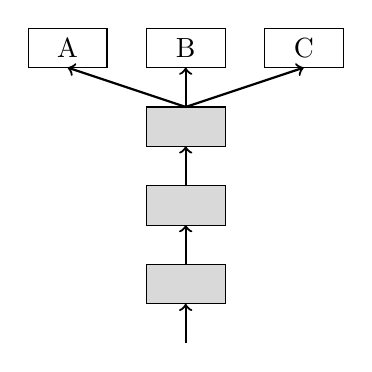
\begin{tikzpicture}
		\begin{scope} [fill opacity = .3]
		\draw [->, thick] (0,0) -- (0, 0.5);
		\draw [fill=gray, draw = black] (-0.5,1) rectangle (0.5, 0.5);
		\draw [->, thick] (0, 1) -- (0, 1.5);
		\draw [fill=gray, draw = black] (-0.5,2) rectangle (0.5, 1.5);
		\draw [->, thick] (0, 2) -- (0, 2.5);
		\draw [fill=gray, draw = black] (-0.5,3) rectangle (0.5, 2.5);
		\draw [draw = black] (-2,4) rectangle (-1, 3.5);
		\draw [draw = black] (-0.5,4) rectangle (0.5, 3.5);
		\draw [draw = black] (1,4) rectangle (2, 3.5);
		\draw [->, thick] (0, 3) -- (-1.5, 3.5);
		\draw [->, thick] (0, 3) -- (0, 3.5);
		\draw [->, thick] (0, 3) -- (1.5, 3.5);
		\end{scope}
		\node at (-1.5, 3.75) {A};
		\node at (0, 3.75) {B};
		\node at (1.5, 3.75) {C};
		
		\end{tikzpicture}
	}
	\hspace{.5in}
	\subfloat[软共享模式]{
		\centering
		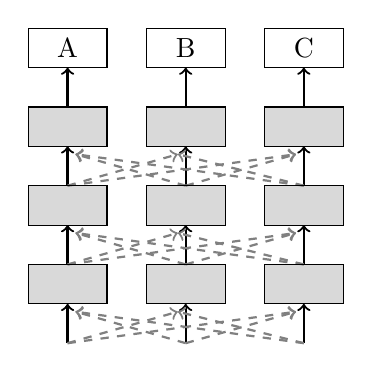
\begin{tikzpicture}
		\begin{scope} [fill opacity = .3]
		\draw [->, thick] (-1.5,0) -- (-1.5, 0.5);
		\draw [->, thick, gray, dashed] (-1.5,0) -- (-.1, 0.4);
		\draw [->, thick, gray, dashed] (-1.5,0) -- (1.4, 0.4);
		
		\draw [->, thick] (-1.5, 1) -- (-1.5, 1.5);
		\draw [->, thick, gray, dashed] (-1.5, 1) -- (-.1, 1.4);
		\draw [->, thick, gray, dashed] (-1.5, 1) -- (1.4, 1.4);
		
		\draw [->, thick] (-1.5, 2) -- (-1.5, 2.5);
		\draw [->, thick, gray, dashed] (-1.5, 2) -- (-.1, 2.4);
		\draw [->, thick, gray, dashed] (-1.5, 2) -- (1.4, 2.4);
		
		\draw [->, thick] (-1.5, 3) -- (-1.5, 3.5);
		
		\draw [fill=gray, draw = black] (-2,1) rectangle (-1, 0.5);
		\draw [fill=gray, draw = black] (-2,2) rectangle (-1, 1.5);
		\draw [fill=gray, draw = black] (-2,3) rectangle (-1, 2.5);
		\draw [draw = black] (-2,4) rectangle (-1, 3.5);
		
		\draw [->, thick] (0,0) -- (0, 0.5);
		\draw [->, thick, gray, dashed] (0,0) -- (-1.4, 0.4);
		\draw [->, thick, gray, dashed] (0,0) -- (1.4, 0.4);
		
		\draw [->, thick] (0, 1) -- (0, 1.5);
		\draw [->, thick, gray, dashed] (0, 1) -- (-1.4, 1.4);
		\draw [->, thick, gray, dashed] (0, 1) -- (1.4, 1.4);
		
		\draw [->, thick] (0, 2) -- (0, 2.5);
		\draw [->, thick, gray, dashed] (0, 2) -- (-1.4, 2.4);
		\draw [->, thick, gray, dashed] (0, 2) -- (1.4, 2.4);
		
		\draw [->, thick] (0, 3) -- (0, 3.5);
		
		\draw [fill=gray, draw = black] (-0.5,1) rectangle (0.5, 0.5);
		\draw [fill=gray, draw = black] (-0.5,2) rectangle (0.5, 1.5);
		\draw [fill=gray, draw = black] (-0.5,3) rectangle (0.5, 2.5);
		\draw [draw = black] (-0.5,4) rectangle (0.5, 3.5);
		
		\draw [->, thick] (1.5, 0) -- (1.5, 0.5);
		\draw [->, thick, gray, dashed] (1.5, 0) -- (-1.4, 0.4);
		\draw [->, thick, gray, dashed] (1.5, 0) -- (-.1, 0.4);
		
		\draw [->, thick] (1.5, 1) -- (1.5, 1.5);
		\draw [->, thick, gray, dashed] (1.5, 1) -- (-1.4, 1.4);
		\draw [->, thick, gray, dashed] (1.5, 1) -- (-.1, 1.4);
		
		\draw [->, thick] (1.5, 2) -- (1.5, 2.5);
		\draw [->, thick, gray, dashed] (1.5, 2) -- (-1.4, 2.4);
		\draw [->, thick, gray, dashed] (1.5, 2) -- (-.1, 2.4);
		
		\draw [->, thick] (1.5, 3) -- (1.5, 3.5);
		
		\draw [fill=gray, draw = black] (1,1) rectangle (2, 0.5);
		\draw [fill=gray, draw = black] (1,2) rectangle (2, 1.5);
		\draw [fill=gray, draw = black] (1,3) rectangle (2, 2.5);
		\draw [ draw = black] (1,4) rectangle (2, 3.5);
		\end{scope}
		\node at (-1.5, 3.75) {A};
		\node at (0, 3.75) {B};
		\node at (1.5, 3.75) {C};
		
		\end{tikzpicture}
	}
	\vspace{.2in}
	
	\subfloat[分层共享模式]{
		\centering
		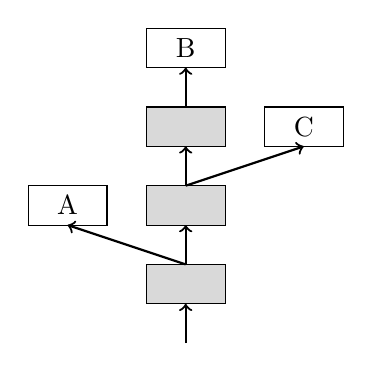
\begin{tikzpicture}
		\begin{scope} [fill opacity = .3]
		\draw [->, thick] (0,0) -- (0, 0.5);
		\draw [->, thick] (0, 1) -- (0, 1.5);
		\draw [->, thick] (0, 2) -- (0, 2.5);
		\draw [->, thick] (0, 3) -- (0, 3.5);
		\draw [->, thick] (0, 1) -- (-1.5, 1.5);
		\draw [->, thick] (0, 2) -- (1.5, 2.5);
		
		\draw [fill=gray, draw = black] (-0.5,1) rectangle (0.5, 0.5);
		\draw [fill=gray, draw = black] (-0.5,2) rectangle (0.5, 1.5);
		\draw [fill=gray, draw = black] (-0.5,3) rectangle (0.5, 2.5);
		
		\draw [ draw = black] (-0.5,4) rectangle (0.5, 3.5);
		\draw [ draw = black] (-2,2) rectangle (-1, 1.5);
		\draw [ draw = black] (1,3) rectangle (2, 2.5);
		\end{scope}
		\node at (-1.5, 1.75) {A};
		\node at (0, 3.75) {B};
		\node at (1.5, 2.75) {C};
		
		\end{tikzpicture}
	}
	\hspace{.5in}
	\subfloat[共享-私有模式]{
		\centering
		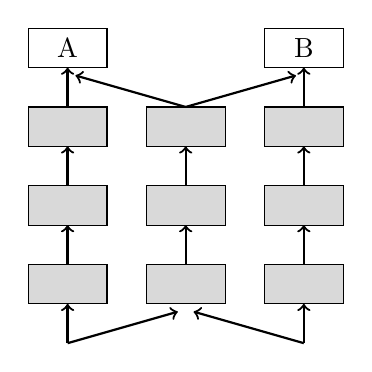
\begin{tikzpicture}
		\begin{scope} [fill opacity = .3]
		\draw [->, thick] (-1.5,0) -- (-1.5, 0.5);
		\draw [->, thick] (-1.5, 1) -- (-1.5, 1.5);
		\draw [->, thick] (-1.5, 2) -- (-1.5, 2.5);
		\draw [->, thick] (-1.5, 3) -- (-1.5, 3.5);
		
		\draw [fill=gray, draw = black] (-2,1) rectangle (-1, 0.5);
		\draw [fill=gray, draw = black] (-2,2) rectangle (-1, 1.5);
		\draw [fill=gray, draw = black] (-2,3) rectangle (-1, 2.5);
		\draw [ draw = black] (-2,4) rectangle (-1, 3.5);
		
		\draw [->, thick] (-1.5,0) -- (-.1, .4);
		\draw [->, thick] (1.5,0) -- (.1, .4);
		\draw [->, thick] (0, 1) -- (0, 1.5);
		\draw [->, thick] (0, 2) -- (0, 2.5);
		\draw [->, thick] (0, 3) -- (-1.4, 3.4);
		\draw [->, thick] (0, 3) -- (1.4, 3.4);
		
		\draw [fill=gray, draw = black] (-0.5,1) rectangle (0.5, 0.5);
		\draw [fill=gray, draw = black] (-0.5,2) rectangle (0.5, 1.5);
		\draw [fill=gray, draw = black] (-0.5,3) rectangle (0.5, 2.5);
		
		\draw [->, thick] (1.5, 0) -- (1.5, 0.5);
		\draw [->, thick] (1.5, 1) -- (1.5, 1.5);
		\draw [->, thick] (1.5, 2) -- (1.5, 2.5);
		\draw [->, thick] (1.5, 3) -- (1.5, 3.5);
		
		\draw [fill=gray, draw = black] (1,1) rectangle (2, 0.5);
		\draw [fill=gray, draw = black] (1,2) rectangle (2, 1.5);
		\draw [fill=gray, draw = black] (1,3) rectangle (2, 2.5);
		\draw [ draw = black] (1,4) rectangle (2, 3.5);
		\end{scope}
		\node at (-1.5, 3.75) {A};
		\node at (1.5, 3.75) {B};
		
		\end{tikzpicture}
	}
	\caption{多任务学习的几种常见共享模式}
	\label{fig:mtl_archs}
\end{figure}

具体的,我们以最常见的硬共享模式为例,给出多任务学习的形式化描述。假设有~$T$~个相关任务,任务~$t$~的数据集为~$\mathcal{D}_t = \lbrace \mathbf{x}_n^{(t)}, y_n^{(t)} \rbrace_{n=1}^{N_t}$,包含~$N_t$~个样本。假设模型在任务~$t$~的第~$n$~个样本上的输出为
\begin{equation}
	\hat{y}_n^{(t)} = \mathcal{G}^{(t)}(\mathcal{F}(\mathbf{x}_n^{(t)}; \theta_\mathcal{F}) ; \theta_{\mathcal{G}^{(t)}}),
\end{equation}
其中~$\mathcal{F}$~为神经网络共享层,$\mathcal{G}^{(t)}$~为任务~$t$~的特定层。模型总参数包含共享层的参数以及任务特定层的参数,即~$\theta = [\theta_\mathcal{F}, \{ \theta_{\mathcal{G}^{(t)}}\}_{t=1}^T]$. 多任务联合学习的损失函数为
\begin{equation}
	\mathcal{L}(\theta) = \sum_{t=1}^T\lambda_t\sum_{n=1}^{N_t}\mathcal{L}_t(\hat{y}_n^{(t)}, y_n^{(t)}),
\end{equation}
其中,$\mathcal{L}_t(\cdot)$~为第~$t$~个任务的损失函数,$\lambda_t$~为第~$t$~个任务损失函数的权重。$\lambda_t$~通常被看作是超参数,根据任务~$t$~的重要程度或困难程度来确定,也可以作为可学习参数根据任务的不确定性来自主学习\cite{DBLP:conf/cvpr/KendallGC18}。

最后,通过优化如下目标来得到模型参数
\begin{equation}
	\theta ^* = \mathop{\arg\min}\limits_{\theta} \mathcal{L}(\theta).
\end{equation}
多任务学习使用的优化算法与常见单任务学习的优化算法没有什么不同,可以采用随机梯度下降等方法。
\section{自然语言处理}
\label{sec:nlp}

\emph{自然语言处理}(Natural Language Processing, NLP)是一门涵盖计算机科学、语言学、数学等多个领域的交叉学科,也是人工智能的核心领域之一,旨在使用计算机技术来处理、理解和生成自然语言文本。同时,自然语言处理也是一个包括词性标注、句法分析、语义角色分析、机器翻译、阅读理解、问答系统、对话系统等在内的庞大的研究领域。从定义上,任何与处理文本数据相关的问题都可以归为自然语言处理的问题。

事实上,人们对NLP的研究早在人工智能被提出之前就开始了。上世纪上半叶,Claude Shannon使用概率模型来描述人类语言,提出用熵来表示语言的不确定性。1956年,Noam Chomsky提出生成语法理论,给出了语言句法结构的符号规则,此后,基于规则的符号系统开始在NLP领域流行。研究人员根据研究工具的不同分为统计和规则两个流派。到上世纪末,随着隐马尔科夫模型、核方法等方法的出现,统计自然语言处理开始因其灵活性和通用性渐渐成为主流。随着深度学习的兴起,这一趋势被再次加强,基于神经网络的方法开始在各大NLP任务上取得~\sArt~结果。

在深度学习背景下,一个使得NLP取得重大进展的关键概念是\emph{分布式表示}(Distributed Representation)\cite{Hinton:1986:DR:104279.104287}。在传统机器学习方法中,普遍采用one-hot方法表示文本特征,即在一向量中用1来表示出现的单词,用0来表示未出现的单词。然而这种表示方法下向量维度与词表大小一致,不便于扩展,且任意两单词之间正交,无法计算语义相似度。而分布式表示则将文本语义分布到向量的各个维度,或者说分布到多个神经元上进行处理。在分布式表示下,文本用低维稠密向量表示,使得语义组合和语义相似度的计算都非常灵活。分布式表示的概念是整个深度学习技术的核心,如何学到一个好的分布式表示是决定各个深度学习算法性能的关键。

在NLP中,文本的分布式表示方法一直是研究重点。分布式表示的应用引出了\emph{词向量}(也被称作\emph{词嵌入})的概念,在词嵌入矩阵中,每个单词用一个低维稠密词向量来表示。最初,Bengio等人\cite{DBLP:conf/nips/BengioDV00}将分布式表示引入语言建模,让神经网络在反向传播时同时更新网络参数和词向量。这里的词向量作为模型的参数,训练前采用随机初始化。2013年,Mikolov等人\cite{DBLP:conf/nips/MikolovSCCD13}提出了word2vec方法,可以在大规模无标注文本上预训练一组词向量,使用预训练的词向量初始化神经网络的词嵌入层可以显著提升模型效果。2014年,Pennington等人\cite{DBLP:conf/emnlp/PenningtonSM14}使用类似的思路发明了GloVe,这种词向量具备更好的线性性质。从此,在绝大多数NLP任务中,人们通常使用预训练好的词向量来作为模型输入,而不再是随机初始化。然而,这些文本表示方法将单词映射为固定的词向量,难以处理一词多义的问题,因此是\emph{未语境化}(non-contextualized)的。在现实场景中,一个词的意思常常要通过其所在的语境来确定,例如“苹果”在某些语境中表示一种水果,而在某些语境中可能表示一家公司。为处理这一问题,人们提出了\emph{语境化}(contextual)的文本表示方法,如ELMo\cite{DBLP:conf/naacl/PetersNIGCLZ18},GPT\cite{radford2018improving},BERT\cite{devlin2018bert}等,这些上下文敏感的文本表示方法使得神经网络模型在各大NLP任务上取得了巨大的提升。

文本的分布式表示一般被认为是神经网络的输入,即第一层(词嵌入层)。为执行特定的任务,通常需要在文本表示的基础上再进行加工得到易于预测的任务特定表示。这种加工可以采用不同的神经网络来实现。在NLP中,目前普遍使用的神经网络为CNN\cite{DBLP:conf/icml/CollobertW08}\cite{DBLP:conf/emnlp/Kim14}\cite{DBLP:conf/icml/GehringAGYD17}和RNN\cite{DBLP:conf/interspeech/MikolovKBCK10}\cite{DBLP:conf/emnlp/WenGMSVY15}\cite{DBLP:conf/acl/MaH16}。然而,这二者还都存在难以解决的缺陷:CNN一般只能建模局部位置信息,难以捕捉长距离句子依赖;而RNN每一时间步的计算都依赖上一时间步的状态,导致其运算速度缓慢,难以并行,无法在大规模工业场景中使用。需要注意的是,本文提到的RNN包含原始版本及其变种,如LSTM\cite{DBLP:journals/neco/GersSC00}和GRU\cite{DBLP:journals/corr/ChungGCB14}.

另外,人们在对自然语言处理、计算机视觉等问题的研究过程中也提出了一些模型无关的机制,其中的一个典型代表就是\emph{注意力机制}。在NLP中,注意力机制最初出现在机器翻译中,显著提升了翻译质量\cite{DBLP:journals/corr/BahdanauCB14}。随后,注意力机制开始在NLP的各个子问题中被广泛使用,基于双向LSTM和注意力机制的神经网络模型一度成为处理包括阅读理解、自然语言推理等在内的各个NLP任务的标配。甚至在2017年,Google提出了完全基于自注意力的神经网络:Transformer\cite{DBLP:conf/nips/VaswaniSPUJGKP17},在机器翻译任务上取得了新的~\sArt~结果。

%\begin{figure}[htb]
%	\centering
%	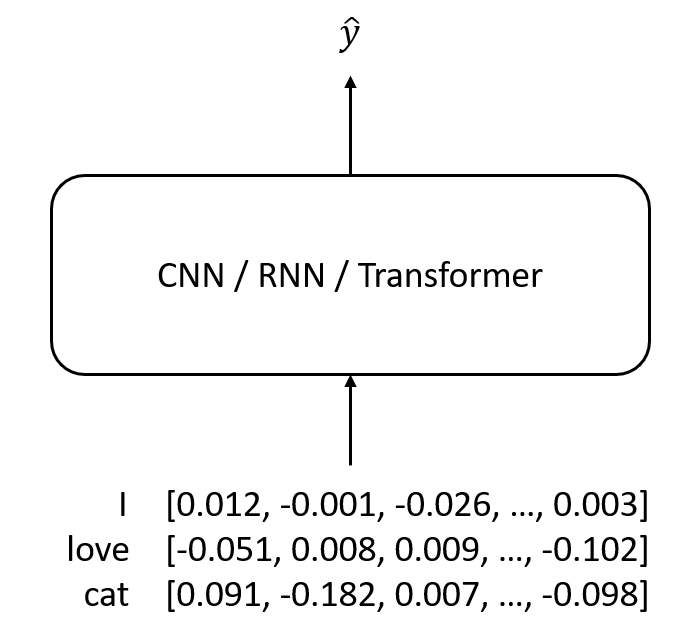
\includegraphics[scale=0.6]{nlp_ppl.png}
%	\caption{基于神经网络处理自然语言的一般模式}
%	\label{fig:nlp_ppl}
%\end{figure}

Transformer在语义信息提取和长距离依赖任务上都取得了富有竞争力的结果\cite{DBLP:conf/emnlp/TangMRS18},并且因其可以并行计算的优点在NLP领域迅速流行。近期,随着基于Transformer的预训练模型BERT\cite{devlin2018bert}取得的巨大成功,Transformer开始受到越来越多的研究者关注,出现了Universal Transformer\cite{dehghani2018universal}、Gaussian Transformer\cite{guo2019gaussian}、Star-Transformer\cite{guo2019star}等变种。

%图~\ref{fig:nlp_ppl}~比较简略地给出了文本从输入神经网络到输出的一般模式。

\section{神经多任务自然语言处理}
\label{sec:mtl4nlp}
在前文中,介绍了深度学习的基本概念,以及多任务学习和自然语言处理在深度学习背景下的研究现状。在这一基础上,本节将介绍基于神经网络的多任务学习在自然语言处理中的主要进展。

事实上,早在十年前就已经有人在神经网络模型中应用多任务学习来解决NLP的问题:Collobert等人\cite{DBLP:conf/icml/CollobertW08}使用一个简单的卷积神经网络(Convolutional Neural Network, CNN)来同时学习词性标注、语块标注、命名实体识别、语义角色标注、语义相似度和语言模型,超越了CNN使用单任务训练时的表现。

随着循环神经网络(Recurrent Neural Network, RNN)在NLP上的广泛应用,研究者开始基于RNN构造多任务学习框架,在机器翻译\cite{DBLP:conf/acl/DongWHYW15}、文本分类\cite{DBLP:conf/ijcai/LiuQH16}\cite{DBLP:conf/acl/LiuQH17}、序列标注\cite{DBLP:conf/acl/SogaardG16}等常见NLP任务上均取得了成功。

图~\ref{fig:mtl_cnn_rnn}~分别给出了多任务学习在CNN和RNN上的两种模型结构:(a) 使用多任务CNN处理词性标注、命名实体识别等多个序列标注任务和语义相似度任务;(b) 使用多任务RNN处理多语言机器翻译问题。两模型均属于多任务学习中的硬共享结构,且(a)模型仅共享词表。

\begin{figure}[htb]
	\centering
	\subfloat[一种多任务CNN模型\cite{DBLP:conf/icml/CollobertW08}]{
		\centering
		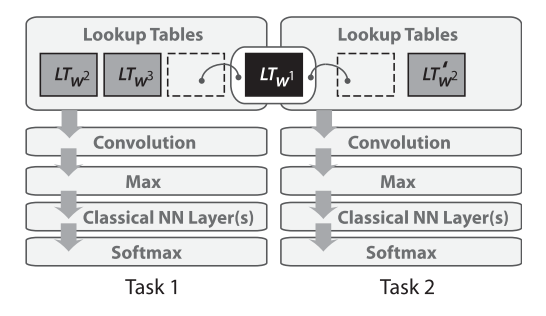
\includegraphics[scale=0.55]{MTL-CNN.PNG}
	}
	\subfloat[一种多任务RNN模型\cite{DBLP:conf/acl/DongWHYW15}]{
		\centering
		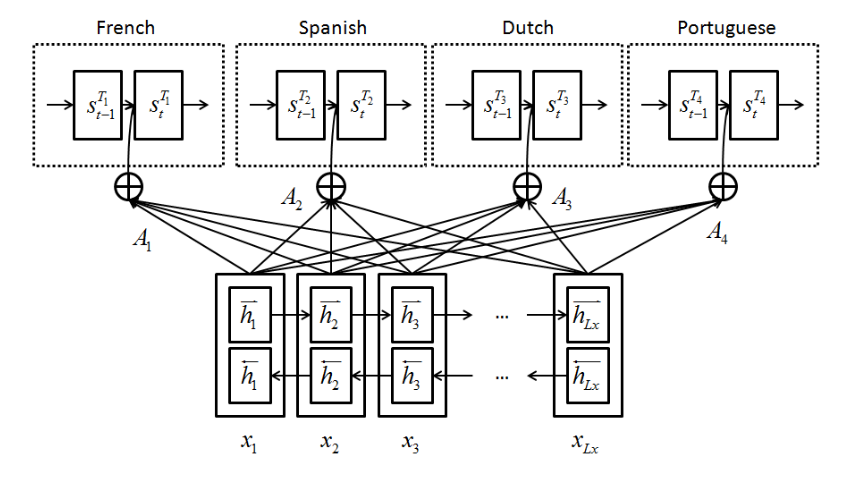
\includegraphics[scale=0.45]{MTL-RNN.PNG}
	}
	\caption{多任务学习在CNN和RNN上的应用示例}
	\label{fig:mtl_cnn_rnn}
\end{figure}

从共享架构上看,基于神经网络的多任务自然语言处理架构涵盖了前文提到的各种共享模式,也出现了一些新颖的共享模式。

首先,最简单的硬共享模式率先在CNN上得到了应用\cite{DBLP:conf/icml/CollobertW08},Dong等人\cite{DBLP:conf/acl/DongWHYW15}又将硬共享模式应用在基于RNN的编码器-解码器框架中来进行多语言机器翻译,将编码器作为共享模块,为每种目标语言设置特定的解码器,该模型可以将源语言同时翻译为多种目标语言,且翻译质量优于使用单任务学习时的效果。Liu等人\cite{DBLP:conf/ijcai/LiuQH16}和Zheng等人\cite{DBLP:conf/ijcai/ZhengCQ18}则将基于硬共享模式的RNN应用在多领域文本分类任务中,前者为每个领域设置不同的输出层,而后者为每个领域使用不同的注意力对共享层特征进行选择。Subramanian等人\cite{DBLP:conf/iclr/SubramanianTBP18}使用包括机器翻译、自然语言推理、成分句法分析等多个句对任务预训练了一个序列到序列的模型,该模型可以作为一个通用句子编码器为下游任务提取句子表示。基于深度学习的硬共享模式简单有效,易于实现,一般无需增加过多参数,直到今天还在作为多任务学习的典型应用模式被广泛使用\cite{liu2019multi}。

然而,硬共享模式由于设置了统一的共享层,限制了多任务共享的灵活性,也限制了共享任务间的跨度,对于弱相关或不相关的任务,硬共享模式甚至可能会损害模型性能。因此,一种更加灵活的共享模式,软共享,随即被应用在NLP问题中。Liu等人\cite{DBLP:conf/ijcai/LiuQH16}提出使用软共享模式的LSTM进行多领域文本分类,具体地,该模型为每一个任务分配一个LSTM层,在执行某一任务时该任务对应的LSTM可以通过门控机制获取其他任务的隐状态信息来形成自己的隐状态。除了使用门控机制对其他任务进行窃听之外,还可以对其他任务特征进行简单的线性加权。Misra等人\cite{DBLP:conf/cvpr/MisraSGH16}基于AlexNet提出了十字缝(cross-stitch)网络来处理多个计算机视觉任务,该网络在池化层和全连接层之间设置十字缝单元,将各任务在某一层得到的特征进行线性组合得到下一层特征。Ruder等人\cite{1705.08142}在十字缝网络的基础上基于RNN提出了水闸网络(Sluice Network)来联合学习词性标注、命名实体识别、语义角色标注等多个NLP任务。

由于NLP任务对文本表示的要求不同,例如比较简单的NLP任务仅需要简单的语法知识而难度较大的任务需要复杂的语义信息,分层共享在RNN中得到了应用。S{\o}gaard等人\cite{DBLP:conf/acl/SogaardG16}使用双向LSTM在词性标注、语块标注和CCG标注三个序列标注任务上进行了实验,结果表明相较于硬共享模式将所有任务放置在同一层的做法,将词性标注这样的低级任务放置在神经网络的低层能够得到更好的效果。Hashimoto等人\cite{DBLP:conf/emnlp/HashimotoXTS17}进一步提出了一种分层多任务学习模型,该模型能够处理更多级别的任务,包含词级别任务(词性标注和语块标注)、语法任务(依存句法分析)和语义任务(语义相似度和文本蕴含任务)。

Liu等人还提出使用基于LSTM的共享-私有模式来解决多领域文本分类问题,其中私有模块可以是LSTM中的内部记忆单元\cite{DBLP:conf/ijcai/LiuQH16},也可以是外部记忆网络\cite{DBLP:conf/emnlp/LiuQH16}。为将共享模块和私有模块的职责分开,避免二者相互干扰,还可以引入对抗训练(Adversarial Training)的方法,训练一任务判别器并使其无法根据共享层的特征分辨当前样本来自哪一个任务,从而得到更纯净的共享表示\cite{DBLP:conf/acl/LiuQH17}。Chen等人\cite{DBLP:journals/corr/abs-1802-08969}将元学习(Meta Learning)方法应用到多任务学习中,使用一个元LSTM作为共享模块来捕捉各任务学习的方式,并用其来控制各任务私有模块的参数。

除了前文提到的四种共享模式之外,在NLP中还出现了很多较新颖的多任务学习模型。例如,Rei\cite{DBLP:conf/acl/Rei17}将语言建模作为辅助任务来增强自己的序列标注模型,Plank等人\cite{DBLP:conf/eacl/PlankA17}和S{\o}gaard等人\cite{DBLP:conf/eacl/SogaardB17}进行了大量实验来探究辅助任务的特点。近年来,随着神经网络架构搜索(Network Architecture Search, NAS)的发展,有人提出多任务共享架构搜索,使用强化学习的方法来自动根据任务和数据的特点选择合适的共享架构\cite{DBLP:journals/corr/abs-1808-07658}。

近期,随着迁移学习在NLP领域取得了巨大成功\cite{DBLP:conf/naacl/PetersNIGCLZ18}\cite{radford2018improving}\cite{devlin2018bert},人们发现学习一个通用的任务无关的表示能够给特定任务带来的收益远远大于根据任务特点对模型结构的改进,这引起了人们对模型的可迁移性和通用性的兴趣。为了评测模型的通用表示能力,研究者们开始关注单一模型在多个任务上的表现,开发出了一些多任务评测基准工具或平台,如SentEval\cite{DBLP:conf/lrec/ConneauK18}、DecaNLP\cite{mccann2018natural}、GLUE\cite{DBLP:conf/emnlp/WangSMHLB18}等。

2018年10月,BERT\cite{devlin2018bert},一个预训练的Transformer模型,在GLUE的多个任务上的表现都大幅度超越了之前的模型。最近,人们发现在BERT的基础上使用多任务学习对模型进行微调能够取得进一步提升\cite{liu2019multi}\cite{anonymous2018bam!}。

BERT的成功证明了Transformer具备强大的共享知识存储能力,然而,相比CNN和RNN,目前还很少有工作探索Transformer上的多任务学习架构。随着Transformer在机器翻译\cite{DBLP:conf/nips/VaswaniSPUJGKP17}、迁移学习\cite{radford2018improving}\cite{devlin2018bert}中取得了巨大成功,如何使其通过多任务学习取得额外的收益,以及如何对其设计新的共享模式都是值得探索的问题。
\chapter{模型}
\label{cha:model}
本章将详细介绍本文所使用的模型,首先在~\ref{sec:tf}~节介绍Google于2017年提出的Transformer,接着在~\ref{sec:mtl_tf}~节介绍多任务Transformer的几种架构,最后在~\ref{sec:imp}~节描述了一些具体的实现细节\footnote{代码见\url{https://github.com/txsun1997/Graduation}}。

\section{Transformer}
\label{sec:tf}
Transformer是Google于2017年提出的一种完全基于\emph{自注意力}(self-attention)的全连接神经网络\cite{DBLP:conf/nips/VaswaniSPUJGKP17},摒弃了之前常用的循环计算和卷积结构,又同时具备了卷积网络的并行计算特性以及循环网络的处理长距离依赖的能力。Transformer最初被用在机器翻译中,因此包含一个\emph{编码器}和一个\emph{解码器},这里仅介绍本文用到的编码器部分\footnote{解码器的构成与编码器十分类似,只是增加了与输入端的注意力交互。}。
\begin{figure}[htb]
	\centering
	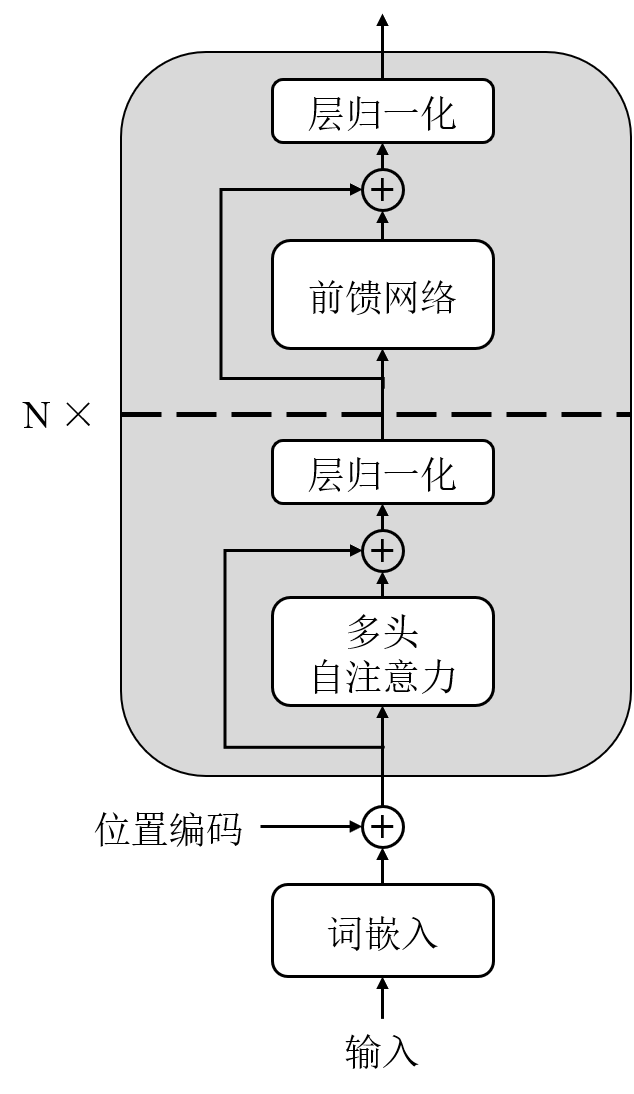
\includegraphics[scale=0.6]{tf.png}
	\caption{Transformer编码器架构}
	\label{fig:tf_encoder}
\end{figure}

作为编码器,Transformer与卷积网络、循环网络的目标一致,都是将输入的句子序列~$(x_1, x_2, ..., x_n)$~映射成一组低维稠密的向量表示~$\mathbf{z} = (\mathbf{z}_1, \mathbf{z}_2, ..., \mathbf{z}_n)$. 其中,每个位置的编码~$\mathbf{z}_i \in \mathbb{R}^{d}$. 给定~$\mathbf{z}$,解码器根据任务的不同生成单个预测~$y$,如文本分类任务,或者多个预测~$(y_1, y_2, ..., y_n)$,如序列标注任务。生成预测的过程通常为使用一线性层再加一\texttt{Softmax}层,即:
\begin{equation}
	\hat{y} = \mathrm{softmax}(\mathbf{z}\mathbf{W} + b).
\end{equation}
其中,$\mathbf{W}\in \mathbb{R}^{d\times c}$,$c$~为类别个数。

Transformer编码器的结构如图~\ref{fig:tf_encoder}~所示,图中阴影部分表示Transformer的一层,左侧的~$N$~表示层数。每一层包含两个子层:第一个子层是一个多头自注意力模块,第二个子层是一个简单的全连接前馈网络。在每个子层都有残差连接\cite{DBLP:conf/cvpr/HeZRS16}和层规一化\cite{lei2016layer}来优化训练过程。因此,每一个子层的输出为~$\mathrm{\texttt{LayerNorm}}(x+\mathrm{\texttt{Sublayer}}(x))$,其中~$\mathrm{\texttt{LayerNorm}}$~为层规范化,$\mathrm{\texttt{Sublayer}}(x)$~表示对应子层实现的函数,即多头自注意力和前馈网络。

下面先介绍第一个子层,该子层主要由多头自注意力模块构成。

\subsection{自注意力}
注意力机制就是把一\emph{查询}向量和一组\emph{键}-\emph{值}对映射为输出,这里的输入、查询(Query)、键(Key)、值(Value)、输出都为向量\footnote{为简便起见,下面的公式中不再对向量加粗表示。}。输出向量由值向量加权得到,每个值向量的权重由查询和键向量计算得出,查询和键向量的计算方式有点积、双线性等形式,Transformer使用的是一种缩放的点积形式。

自注意力是指查询、键、值都出自输入本身。假设有一个向量序列输入~$H = [h_1, \hdots, h_n]^\top \in \mathbb{R}^{n\times d}$,其中~$n$~为句子长度,$d$~为输入维度,则自注意力的计算方式为:
\begin{equation}
	\mathrm{Attention}(Q,K,V) = \mathrm{softmax}(\frac{QK^\top}{\sqrt{d_k}}V)
\end{equation}
其中,$Q=HW^Q, K=HW^K, V=HW^V$\ 且\ $W^Q, W^K, W^V\in \mathbb{R}^{d\times d_k}$. 

\subsection{多头自注意力}
为了捕获更丰富的语义模式,提取句子元素之间更多的交互信息,Transformer使用了\emph{多头自注意力}(multi-head self-attention)机制:
\begin{equation}
	\begin{aligned}
	\mathrm{MultiHead}(Q,K,V)& = \mathrm{Concat}(\mathrm{head_1}, \hdots, \mathrm{head_h})W^O
	\\
	\mathrm{head_i} &= \mathrm{Attention}(HW_i^Q, HW_i^K, HW_i^V).
	\end{aligned}
\end{equation}
这里,每个头的维度就是~$d_k$,输出矩阵~$W^O\in \mathbb{R}^{d_kh \times d}$. 在提出Transformer的论文中,作者设置~$d_k=d/h$,即令隐层维度被头的个数整除。

\subsection{前馈网络}
第二个子层主要由一单隐层全连接前馈网络构成,其输入为第一个子层的输出。假设第一个子层的输出为~$x\in \mathbb{R}^{n\times d}$,则前馈网络的输出为:
\begin{equation}
	\mathrm{FFN}(x) = \max(0, xW_1+b_1)W_2+b_2.
\end{equation}
其中,$W_1 \in \mathbb{R}^{d\times d_{ff}}, W_2 \in \mathbb{R}^{d_{ff} \times d}$,$d_{ff}$~为前馈网络的隐层神经元个数。前馈网络的隐层使用的激活函数为ReLU函数,即~$\mathrm{ReLU}(\cdot)=\max(0, \cdot)$.

\subsection{位置编码}
由于Transformer完全使用自注意力机制来对输入句子进行建模,无法将时序关系考虑进去,例如,对于不使用位置编码的Transformer来说,“猫坐在椅子上”和“椅子坐在猫上”两句话的表示并没有什么不同。因此需要在输入时加入额外的\emph{位置编码}(position encoding)。通常来说,加入位置编码有两种方式:一种是作为可学习的参数让模型自己学到,另一种是人为地设计对位置和维度都敏感的编码函数,例如:
\begin{equation}
	\begin{aligned}
	\mathrm{PE}_{(pos, 2i)} &= \sin(pos/10000^{2i/d})\\
	\mathrm{PE}_{(pos, 2i+1)} &= \cos(pos/10000^{2i/d})
	\end{aligned}
\end{equation}
其中,$pos$表示记号在句子中的位置,$i$表示向量维度。

最终,句中每个单词的表示由词向量与位置编码相加组成,词向量可以随机初始化,也可以使用预训练好的词向量,如word2vec,GloVe等。

至此,我们详细描述了Transformer的结构以及输入输出。容易发现,Transformer实际上就是利用注意力机制来建模句子中任意单词与其他单词之间的关系,是一种全连接的全局建模方法。不同于传统的全连接网络,Transformer可以处理变长的句子,因为连接权重是根据输入单词来动态生成的。考虑到这种建模方式,可以给出一个Transformer架构的简化图~\ref{fig:tf_simp},下一节中也将基于类似的简化图来描述我们的多任务Transformer结构。

\begin{figure}[htb]
	\centering
	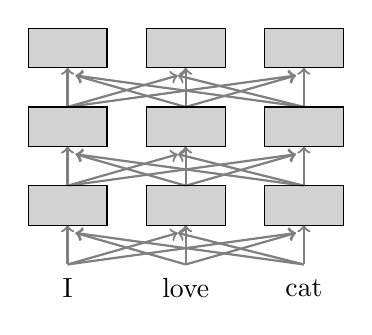
\begin{tikzpicture}
	\begin{scope}[fill opacity = .7]
	\draw [->, thick, gray ] (-1.5,0) -- (-1.5, 0.5);
	\draw [->, thick, gray ] (-1.5,0) -- (-.1, 0.4);
	\draw [->, thick, gray ] (-1.5,0) -- (1.4, 0.4);
	
	\draw [->, thick, gray ] (-1.5, 1) -- (-1.5, 1.5);
	\draw [->, thick, gray ] (-1.5, 1) -- (-.1, 1.4);
	\draw [->, thick, gray ] (-1.5, 1) -- (1.4, 1.4);
	
	\draw [->, thick, gray ] (-1.5, 2) -- (-1.5, 2.5);
	\draw [->, thick, gray ] (-1.5, 2) -- (-.1, 2.4);
	\draw [->, thick, gray ] (-1.5, 2) -- (1.4, 2.4);
	
	\draw [fill=lightgray, draw = black] (-2,1) rectangle (-1, 0.5);
	\draw [fill=lightgray, draw = black] (-2,2) rectangle (-1, 1.5);
	\draw [fill=lightgray, draw = black] (-2,3) rectangle (-1, 2.5);
	
	\draw [->, thick, gray ] (0,0) -- (0, 0.5);
	\draw [->, thick, gray ] (0,0) -- (-1.4, 0.4);
	\draw [->, thick, gray ] (0,0) -- (1.4, 0.4);
	
	\draw [->, thick, gray ] (0, 1) -- (0, 1.5);
	\draw [->, thick, gray ] (0, 1) -- (-1.4, 1.4);
	\draw [->, thick, gray ] (0, 1) -- (1.4, 1.4);
	
	\draw [->, thick, gray ] (0, 2) -- (0, 2.5);
	\draw [->, thick, gray ] (0, 2) -- (-1.4, 2.4);
	\draw [->, thick, gray ] (0, 2) -- (1.4, 2.4);
	
	\draw [fill=lightgray, draw = black] (-0.5,1) rectangle (0.5, 0.5);
	\draw [fill=lightgray, draw = black] (-0.5,2) rectangle (0.5, 1.5);
	\draw [fill=lightgray, draw = black] (-0.5,3) rectangle (0.5, 2.5);
	
	\draw [->, thick, gray ] (1.5, 0) -- (1.5, 0.5);
	\draw [->, thick, gray ] (1.5, 0) -- (-1.4, 0.4);
	\draw [->, thick, gray ] (1.5, 0) -- (-.1, 0.4);
	
	\draw [->, thick, gray ] (1.5, 1) -- (1.5, 1.5);
	\draw [->, thick, gray ] (1.5, 1) -- (-1.4, 1.4);
	\draw [->, thick, gray ] (1.5, 1) -- (-.1, 1.4);
	
	\draw [->, thick, gray ] (1.5, 2) -- (1.5, 2.5);
	\draw [->, thick, gray ] (1.5, 2) -- (-1.4, 2.4);
	\draw [->, thick, gray ] (1.5, 2) -- (-.1, 2.4);
	
	\draw [fill=lightgray, draw = black] (1,1) rectangle (2, 0.5);
	\draw [fill=lightgray, draw = black] (1,2) rectangle (2, 1.5);
	\draw [fill=lightgray, draw = black] (1,3) rectangle (2, 2.5);
	
	\end{scope}
	\node at (0, -.3) {love};
	\node at (-1.5, -.3) {I};
	\node at (1.5, -.3) {cat};
	\end{tikzpicture}
	\caption{Transformer结构的一个简化版示意图}
	\label{fig:tf_simp}
\end{figure}

\section{多任务Transformer}
\label{sec:mtl_tf}
在前文基础上,本节将展示四种基于Transformer的共享架构,其中两种为传统的硬共享模式,由于这种架构的任务特定层堆叠在共享层上面,在神经网络的顶层形成不同任务的表示,因此我们将其归纳为\emph{顶层分化};另外两种为针对Transformer的结构特点提出的共享模式,我们称之为\emph{逐层分化},即在每一层都形成任务特定表示。

对于顶层分化模式,我们给出了两种具体的实现结构:S-P结构和S-C结构。对于逐层分化模式,我们也给出了两种架构方式:L-I结构和L-E结构。

\subsection{S-P结构}
S-P意为Stack-Pooling,即\emph{堆叠-汇聚结构}。S-P结构是指在Transformer的共享层上使用信息汇聚(也称池化)的方式来得到通用句子表示。池化方式一般有两种:\emph{平均池化}(mean pooling)和\emph{最大池化}(max pooling)。以平均池化为例,假设包含~$n$~个单词的句子输入为~$x$,经过Transformer共享层之后输出的隐状态为~$z = \mathcal{F}(x) \in \mathbb{R}^{n \times d}$,则平均池化S-P结构的预测为
\begin{equation}
	\hat{y} = \mathrm{softmax}(\frac{1}{n}\sum_{i=1}^{n}z_i\cdot W^{(t)} + b).
	\label{eq:s-p}
\end{equation}
其中任务~$t$的分类矩阵~$W^{(t)}\in \mathbb{R}^{d\times c}$,$c$~为分类个数。在实际实现时,平均池化后先接一多层感知机(MLP)再输入\texttt{softmax}常常能取得更好的效果,此时式~\ref{eq:s-p}~可写为
\begin{equation}
	\hat{y} = \mathrm{softmax}(\mathrm{MLP}(\frac{1}{n}\sum_{i=1}^{n}z_i)).
\end{equation}

图~\ref{fig:s-p}~给出了S-P结构的示意,与~\ref{sec:mtl}~节的设定相同,浅灰色模块表示共享部分,深灰色模块代表整个句子的表示,$A,B,C$~代表三个不同的任务。

\begin{figure}[htb]
	\centering
	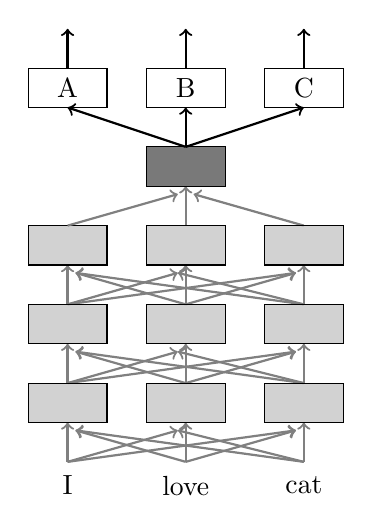
\begin{tikzpicture}
	\begin{scope}[fill opacity = .7]
	\draw [->, thick, gray ] (-1.5,0) -- (-1.5, 0.5);
	\draw [->, thick, gray ] (-1.5,0) -- (-.1, 0.4);
	\draw [->, thick, gray ] (-1.5,0) -- (1.4, 0.4);
	
	\draw [->, thick, gray ] (-1.5, 1) -- (-1.5, 1.5);
	\draw [->, thick, gray ] (-1.5, 1) -- (-.1, 1.4);
	\draw [->, thick, gray ] (-1.5, 1) -- (1.4, 1.4);
	
	\draw [->, thick, gray ] (-1.5, 2) -- (-1.5, 2.5);
	\draw [->, thick, gray ] (-1.5, 2) -- (-.1, 2.4);
	\draw [->, thick, gray ] (-1.5, 2) -- (1.4, 2.4);
	
	\draw [fill=lightgray, draw = black] (-2,1) rectangle (-1, 0.5);
	\draw [fill=lightgray, draw = black] (-2,2) rectangle (-1, 1.5);
	\draw [fill=lightgray, draw = black] (-2,3) rectangle (-1, 2.5);
	
	\draw [->, thick, gray ] (0,0) -- (0, 0.5);
	\draw [->, thick, gray ] (0,0) -- (-1.4, 0.4);
	\draw [->, thick, gray ] (0,0) -- (1.4, 0.4);
	
	\draw [->, thick, gray ] (0, 1) -- (0, 1.5);
	\draw [->, thick, gray ] (0, 1) -- (-1.4, 1.4);
	\draw [->, thick, gray ] (0, 1) -- (1.4, 1.4);
	
	\draw [->, thick, gray ] (0, 2) -- (0, 2.5);
	\draw [->, thick, gray ] (0, 2) -- (-1.4, 2.4);
	\draw [->, thick, gray ] (0, 2) -- (1.4, 2.4);
	
	\draw [->, thick, gray ] (0, 3) -- (0, 3.5);
	\draw [->, thick, gray ] (-1.5, 3) -- (-.1, 3.4);
	\draw [->, thick, gray ] (1.5, 3) -- (.1, 3.4);
	
	\draw [fill=lightgray, draw = black] (-0.5,1) rectangle (0.5, 0.5);
	\draw [fill=lightgray, draw = black] (-0.5,2) rectangle (0.5, 1.5);
	\draw [fill=lightgray, draw = black] (-0.5,3) rectangle (0.5, 2.5);
	\draw [fill=darkgray, draw = black] (-0.5,4) rectangle (0.5, 3.5);
	
	\draw [->, thick, gray ] (1.5, 0) -- (1.5, 0.5);
	\draw [->, thick, gray ] (1.5, 0) -- (-1.4, 0.4);
	\draw [->, thick, gray ] (1.5, 0) -- (-.1, 0.4);
	
	\draw [->, thick, gray ] (1.5, 1) -- (1.5, 1.5);
	\draw [->, thick, gray ] (1.5, 1) -- (-1.4, 1.4);
	\draw [->, thick, gray ] (1.5, 1) -- (-.1, 1.4);
	
	\draw [->, thick, gray ] (1.5, 2) -- (1.5, 2.5);
	\draw [->, thick, gray ] (1.5, 2) -- (-1.4, 2.4);
	\draw [->, thick, gray ] (1.5, 2) -- (-.1, 2.4);
	
	\draw [fill=lightgray, draw = black] (1,1) rectangle (2, 0.5);
	\draw [fill=lightgray, draw = black] (1,2) rectangle (2, 1.5);
	\draw [fill=lightgray, draw = black] (1,3) rectangle (2, 2.5);
	
	\draw [draw = black] (-2,5) rectangle (-1, 4.5);
	\draw [draw = black] (-.5,5) rectangle (.5, 4.5);
	\draw [draw = black] (1,5) rectangle (2, 4.5);
	
	\draw [->, thick] (0, 4) -- (0, 4.5);
	\draw [->, thick] (0, 4) -- (-1.5, 4.5);
	\draw [->, thick] (0, 4) -- (1.5, 4.5);
	
	\draw [->, thick] (0, 5) -- (0, 5.5);
	\draw [->, thick] (-1.5, 5) -- (-1.5, 5.5);
	\draw [->, thick] (1.5, 5) -- (1.5, 5.5);
	
	\end{scope}
	\node at (0, -.3) {love};
	\node at (-1.5, -.3) {I};
	\node at (1.5, -.3) {cat};
	
	\node at (-1.5, 4.75) {A};
	\node at (0, 4.75) {B};
	\node at (1.5, 4.75) {C};
	
	\end{tikzpicture}
	\caption{Stack-Pooling结构}
	\label{fig:s-p}
\end{figure}

\subsection{S-C结构}
S-C意为Stack-CLS,即\emph{堆叠-CLS结构}。S-C结构是指在Transformer的输入时添加一个\texttt{CLS}记号用来捕捉句子在每一层的表示,最后使用\texttt{CLS}的顶层表示来作为句子的通用表示。\texttt{CLS}为Classification的简写,该方法与\cite{devlin2018bert}中的设置一致。

假设最顶层的\texttt{CLS}的表示为~$z_{CLS}\in \mathbb{R}^d$,则S-C结构的输出为
\begin{equation}
	\hat{y} = \mathrm{softmax}(z_{CLS}\cdot W^{(t)} + b).
	\label{eq:cls}
\end{equation}
其中任务~$t$~的分类矩阵~$W^{(t)}\in \mathbb{R}^{d\times c}$,$c$~为分类个数。图~\ref{fig:s-c}~给出了S-C结构的示意图,浅灰色为共享模块,深灰色为共享句子表示。

\begin{figure}[htb]
	\centering
	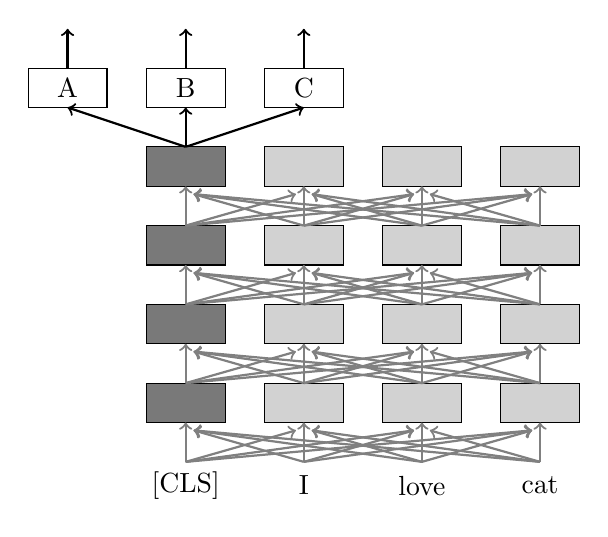
\begin{tikzpicture}
	\begin{scope}[fill opacity = .7]
	
	\draw [->, thick] (-3, 5) -- (-3, 5.5);
	\draw [->, thick] (0, 5) -- (0, 5.5);
	\draw [->, thick] (-1.5, 5) -- (-1.5, 5.5);
	
	% 中间一列
	% modules
	\draw [fill=lightgray, draw = black] (-.5, 1) rectangle (.5, .5);
	\draw [fill=lightgray, draw = black] (-.5, 2) rectangle (.5, 1.5);
	\draw [fill=lightgray, draw = black] (-.5, 3) rectangle (.5, 2.5);
	\draw [fill=lightgray, draw = black] (-.5, 4) rectangle (.5, 3.5);
	\draw [draw = black] (-.5, 5) rectangle (.5, 4.5);
	% lines
	\draw [->, thick, gray ] (0, 0) -- (0, .5);
	\draw [->, thick, gray ] (0, 0) -- (-1.4, .4);
	\draw [->, thick, gray ] (0, 0) -- (1.4, .4);
	\draw [->, thick, gray ] (0, 0) -- (2.9, .4);
	
	\draw [->, thick, gray ] (0, 1) -- (0, 1.5);
	\draw [->, thick, gray ] (0, 1) -- (-1.4, 1.4);
	\draw [->, thick, gray ] (0, 1) -- (1.4, 1.4);
	\draw [->, thick, gray ] (0, 1) -- (2.9, 1.4);
	
	\draw [->, thick, gray ] (0, 2) -- (0, 2.5);
	\draw [->, thick, gray ] (0, 2) -- (-1.4, 2.4);
	\draw [->, thick, gray ] (0, 2) -- (1.4, 2.4);
	\draw [->, thick, gray ] (0, 2) -- (2.9, 2.4);
	
	\draw [->, thick, gray ] (0, 3) -- (0, 3.5);
	\draw [->, thick, gray ] (0, 3) -- (-1.4, 3.4);
	\draw [->, thick, gray ] (0, 3) -- (1.4, 3.4);
	\draw [->, thick, gray ] (0, 3) -- (2.9, 3.4);
	
	\draw [->, thick] (-1.5, 4) -- (0, 4.5);
	
	% 左二
	% modules
	\draw [fill=darkgray, draw = black] (-2, 1) rectangle (-1, .5);
	\draw [fill=darkgray, draw = black] (-2, 2) rectangle (-1, 1.5);
	\draw [fill=darkgray, draw = black] (-2, 3) rectangle (-1, 2.5);
	\draw [fill=darkgray, draw = black] (-2, 4) rectangle (-1, 3.5);
	\draw [draw = black] (-2, 5) rectangle (-1, 4.5);
	% lines
	\draw [->, thick, gray ] (-1.5, 0) -- (-1.5, .5);
	\draw [->, thick, gray ] (-1.5, 0) -- (-.1, .4);
	\draw [->, thick, gray ] (-1.5, 0) -- (1.4, .4);
	\draw [->, thick, gray ] (-1.5, 0) -- (2.9, .4);
	
	\draw [->, thick, gray ] (-1.5, 1) -- (-1.5, 1.5);
	\draw [->, thick, gray ] (-1.5, 1) -- (-.1, 1.4);
	\draw [->, thick, gray ] (-1.5, 1) -- (1.4, 1.4);
	\draw [->, thick, gray ] (-1.5, 1) -- (2.9, 1.4);
	
	\draw [->, thick, gray ] (-1.5, 2) -- (-1.5, 2.5);
	\draw [->, thick, gray ] (-1.5, 2) -- (-.1, 2.4);
	\draw [->, thick, gray ] (-1.5, 2) -- (1.4, 2.4);
	\draw [->, thick, gray ] (-1.5, 2) -- (2.9, 2.4);
	
	\draw [->, thick, gray ] (-1.5, 3) -- (-1.5, 3.5);
	\draw [->, thick, gray ] (-1.5, 3) -- (-.1, 3.4);
	\draw [->, thick, gray ] (-1.5, 3) -- (1.4, 3.4);
	\draw [->, thick, gray ] (-1.5, 3) -- (2.9, 3.4);
	
	\draw [->, thick] (-1.5, 4) -- (-1.5, 4.5);
	
	% 最左
	% modules
	\draw [draw = black] (-3.5, 5) rectangle (-2.5, 4.5);
	% lines
	\draw [->, thick] (-1.5, 4) -- (-3, 4.5);
	
	% 右2
	% modules
	\draw [fill=lightgray, draw = black] (1, 1) rectangle (2, .5);
	\draw [fill=lightgray, draw = black] (1, 2) rectangle (2, 1.5);
	\draw [fill=lightgray, draw = black] (1, 3) rectangle (2, 2.5);
	\draw [fill=lightgray, draw = black] (1, 4) rectangle (2, 3.5);
	% lines
	\draw [->, thick, gray ] (1.5, 0) -- (1.5, .5);
	\draw [->, thick, gray ] (1.5, 0) -- (-1.4, .4);
	\draw [->, thick, gray ] (1.5, 0) -- (.1, .4);
	\draw [->, thick, gray ] (1.5, 0) -- (2.9, .4);
	
	\draw [->, thick, gray ] (1.5, 1) -- (1.5, 1.5);
	\draw [->, thick, gray ] (1.5, 1) -- (-1.4, 1.4);
	\draw [->, thick, gray ] (1.5, 1) -- (.1, 1.4);
	\draw [->, thick, gray ] (1.5, 1) -- (2.9, 1.4);
	
	\draw [->, thick, gray ] (1.5, 2) -- (1.5, 2.5);
	\draw [->, thick, gray ] (1.5, 2) -- (-1.4, 2.4);
	\draw [->, thick, gray ] (1.5, 2) -- (.1, 2.4);
	\draw [->, thick, gray ] (1.5, 2) -- (2.9, 2.4);
	
	\draw [->, thick, gray ] (1.5, 3) -- (1.5, 3.5);
	\draw [->, thick, gray ] (1.5, 3) -- (-1.4, 3.4);
	\draw [->, thick, gray ] (1.5, 3) -- (.1, 3.4);
	\draw [->, thick, gray ] (1.5, 3) -- (2.9, 3.4);
	
	
	% 最右
	% modules
	\draw [fill=lightgray, draw = black] (2.5, 1) rectangle (3.5, .5);
	\draw [fill=lightgray, draw = black] (2.5, 2) rectangle (3.5, 1.5);
	\draw [fill=lightgray, draw = black] (2.5, 3) rectangle (3.5, 2.5);
	\draw [fill=lightgray, draw = black] (2.5, 4) rectangle (3.5, 3.5);
	% lines
	\draw [->, thick, gray ] (3, 0) -- (3, .5);
	\draw [->, thick, gray ] (3, 0) -- (-1.4, .4);
	\draw [->, thick, gray ] (3, 0) -- (.1, .4);
	\draw [->, thick, gray ] (3, 0) -- (1.6, .4);
	
	\draw [->, thick, gray ] (3, 1) -- (3, 1.5);
	\draw [->, thick, gray ] (3, 1) -- (-1.4, 1.4);
	\draw [->, thick, gray ] (3, 1) -- (.1, 1.4);
	\draw [->, thick, gray ] (3, 1) -- (1.6, 1.4);
	
	\draw [->, thick, gray ] (3, 2) -- (3, 2.5);
	\draw [->, thick, gray ] (3, 2) -- (-1.4, 2.4);
	\draw [->, thick, gray ] (3, 2) -- (.1, 2.4);
	\draw [->, thick, gray ] (3, 2) -- (1.6, 2.4);
	
	\draw [->, thick, gray ] (3, 3) -- (3, 3.5);
	\draw [->, thick, gray ] (3, 3) -- (-1.4, 3.4);
	\draw [->, thick, gray ] (3, 3) -- (.1, 3.4);
	\draw [->, thick, gray ] (3, 3) -- (1.6, 3.4);
	
	\end{scope}
	
	% 输入句子
	\node at (-1.5, -.3) {[CLS]};
	\node at (0, -.3) {I};
	\node at (1.5, -.3) {love};
	\node at (3, -.3) {cat};
	
	% 任务特定层
	\node at (-3, 4.75) {A};
	\node at (-1.5, 4.75) {B};
	\node at (0, 4.75) {C};
	\end{tikzpicture}
	\caption{Stack-CLS结构}
	\label{fig:s-c}
\end{figure}

然而,在神经网络顶层形成的句子表示上进行分化得到任务特定表示的方法限制了任务特定表示对底层语义信息的使用。不同任务关注的句子信息可能在语法和语义层面都非常不同,为鼓励不同任务表示的差异化,可以在每一层都形成任务特定的表示,这就是逐层分化模式。下面介绍该模式的两种实现结构:L-I结构和L-E结构。

\subsection{L-I结构}
L-I意为Layerwise-Implicit,即\emph{层级-隐式共享结构}。首先,L-I结构将原来的\texttt{CLS}记号替换为\texttt{TASK},该记号表示任务编号,每个任务编号对应一个不同的任务向量。同时,在L-I结构中,若不同任务的类别数相同,可以不再单独设置任务特定层,不同任务通过输入不同的任务编号\texttt{TASK}来控制。

在L-I结构中,不同任务之间无法显式地交互,只能通过共享模块来隐式地交互,但不同任务在每一层都有自己的表示,因而称为层级隐式共享。L-I结构如图~\ref{fig:l-i}~所示。

\begin{figure}[htb]
	\centering
	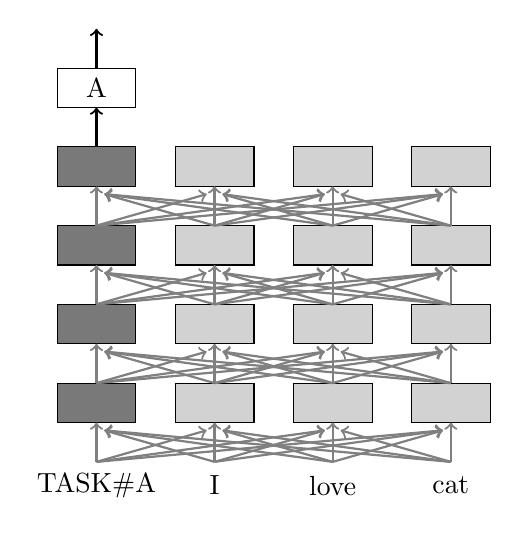
\begin{tikzpicture}
	\node at (-1.5, 4.75) {A};
	\begin{scope}[fill opacity = .7]
	
	\draw [->, thick] (-1.5, 5) -- (-1.5, 5.5);
	
	% 中间一列
	% modules
	\draw [fill=lightgray, draw = black] (-.5, 1) rectangle (.5, .5);
	\draw [fill=lightgray, draw = black] (-.5, 2) rectangle (.5, 1.5);
	\draw [fill=lightgray, draw = black] (-.5, 3) rectangle (.5, 2.5);
	\draw [fill=lightgray, draw = black] (-.5, 4) rectangle (.5, 3.5);
	% lines
	\draw [->, thick, gray ] (0, 0) -- (0, .5);
	\draw [->, thick, gray ] (0, 0) -- (-1.4, .4);
	\draw [->, thick, gray ] (0, 0) -- (1.4, .4);
	\draw [->, thick, gray ] (0, 0) -- (2.9, .4);
	
	\draw [->, thick, gray ] (0, 1) -- (0, 1.5);
	\draw [->, thick, gray ] (0, 1) -- (-1.4, 1.4);
	\draw [->, thick, gray ] (0, 1) -- (1.4, 1.4);
	\draw [->, thick, gray ] (0, 1) -- (2.9, 1.4);
	
	\draw [->, thick, gray ] (0, 2) -- (0, 2.5);
	\draw [->, thick, gray ] (0, 2) -- (-1.4, 2.4);
	\draw [->, thick, gray ] (0, 2) -- (1.4, 2.4);
	\draw [->, thick, gray ] (0, 2) -- (2.9, 2.4);
	
	\draw [->, thick, gray ] (0, 3) -- (0, 3.5);
	\draw [->, thick, gray ] (0, 3) -- (-1.4, 3.4);
	\draw [->, thick, gray ] (0, 3) -- (1.4, 3.4);
	\draw [->, thick, gray ] (0, 3) -- (2.9, 3.4);
	
	% 左二
	% modules
	\draw [fill=darkgray, draw = black] (-2, 1) rectangle (-1, .5);
	\draw [fill=darkgray, draw = black] (-2, 2) rectangle (-1, 1.5);
	\draw [fill=darkgray, draw = black] (-2, 3) rectangle (-1, 2.5);
	\draw [fill=darkgray, draw = black] (-2, 4) rectangle (-1, 3.5);
	\draw [draw = black] (-2, 5) rectangle (-1, 4.5);
	
	% lines
	\draw [->, thick, gray ] (-1.5, 0) -- (-1.5, .5);
	\draw [->, thick, gray ] (-1.5, 0) -- (-.1, .4);
	\draw [->, thick, gray ] (-1.5, 0) -- (1.4, .4);
	\draw [->, thick, gray ] (-1.5, 0) -- (2.9, .4);
	
	\draw [->, thick, gray ] (-1.5, 1) -- (-1.5, 1.5);
	\draw [->, thick, gray ] (-1.5, 1) -- (-.1, 1.4);
	\draw [->, thick, gray ] (-1.5, 1) -- (1.4, 1.4);
	\draw [->, thick, gray ] (-1.5, 1) -- (2.9, 1.4);
	
	\draw [->, thick, gray ] (-1.5, 2) -- (-1.5, 2.5);
	\draw [->, thick, gray ] (-1.5, 2) -- (-.1, 2.4);
	\draw [->, thick, gray ] (-1.5, 2) -- (1.4, 2.4);
	\draw [->, thick, gray ] (-1.5, 2) -- (2.9, 2.4);
	
	\draw [->, thick, gray ] (-1.5, 3) -- (-1.5, 3.5);
	\draw [->, thick, gray ] (-1.5, 3) -- (-.1, 3.4);
	\draw [->, thick, gray ] (-1.5, 3) -- (1.4, 3.4);
	\draw [->, thick, gray ] (-1.5, 3) -- (2.9, 3.4);
	
	\draw [->, thick] (-1.5, 4) -- (-1.5, 4.5);
	
	% 右2
	% modules
	\draw [fill=lightgray, draw = black] (1, 1) rectangle (2, .5);
	\draw [fill=lightgray, draw = black] (1, 2) rectangle (2, 1.5);
	\draw [fill=lightgray, draw = black] (1, 3) rectangle (2, 2.5);
	\draw [fill=lightgray, draw = black] (1, 4) rectangle (2, 3.5);
	% lines
	\draw [->, thick, gray ] (1.5, 0) -- (1.5, .5);
	\draw [->, thick, gray ] (1.5, 0) -- (-1.4, .4);
	\draw [->, thick, gray ] (1.5, 0) -- (.1, .4);
	\draw [->, thick, gray ] (1.5, 0) -- (2.9, .4);
	
	\draw [->, thick, gray ] (1.5, 1) -- (1.5, 1.5);
	\draw [->, thick, gray ] (1.5, 1) -- (-1.4, 1.4);
	\draw [->, thick, gray ] (1.5, 1) -- (.1, 1.4);
	\draw [->, thick, gray ] (1.5, 1) -- (2.9, 1.4);
	
	\draw [->, thick, gray ] (1.5, 2) -- (1.5, 2.5);
	\draw [->, thick, gray ] (1.5, 2) -- (-1.4, 2.4);
	\draw [->, thick, gray ] (1.5, 2) -- (.1, 2.4);
	\draw [->, thick, gray ] (1.5, 2) -- (2.9, 2.4);
	
	\draw [->, thick, gray ] (1.5, 3) -- (1.5, 3.5);
	\draw [->, thick, gray ] (1.5, 3) -- (-1.4, 3.4);
	\draw [->, thick, gray ] (1.5, 3) -- (.1, 3.4);
	\draw [->, thick, gray ] (1.5, 3) -- (2.9, 3.4);
	
	
	% 最右
	% modules
	\draw [fill=lightgray, draw = black] (2.5, 1) rectangle (3.5, .5);
	\draw [fill=lightgray, draw = black] (2.5, 2) rectangle (3.5, 1.5);
	\draw [fill=lightgray, draw = black] (2.5, 3) rectangle (3.5, 2.5);
	\draw [fill=lightgray, draw = black] (2.5, 4) rectangle (3.5, 3.5);
	% lines
	\draw [->, thick, gray ] (3, 0) -- (3, .5);
	\draw [->, thick, gray ] (3, 0) -- (-1.4, .4);
	\draw [->, thick, gray ] (3, 0) -- (.1, .4);
	\draw [->, thick, gray ] (3, 0) -- (1.6, .4);
	
	\draw [->, thick, gray ] (3, 1) -- (3, 1.5);
	\draw [->, thick, gray ] (3, 1) -- (-1.4, 1.4);
	\draw [->, thick, gray ] (3, 1) -- (.1, 1.4);
	\draw [->, thick, gray ] (3, 1) -- (1.6, 1.4);
	
	\draw [->, thick, gray ] (3, 2) -- (3, 2.5);
	\draw [->, thick, gray ] (3, 2) -- (-1.4, 2.4);
	\draw [->, thick, gray ] (3, 2) -- (.1, 2.4);
	\draw [->, thick, gray ] (3, 2) -- (1.6, 2.4);
	
	\draw [->, thick, gray ] (3, 3) -- (3, 3.5);
	\draw [->, thick, gray ] (3, 3) -- (-1.4, 3.4);
	\draw [->, thick, gray ] (3, 3) -- (.1, 3.4);
	\draw [->, thick, gray ] (3, 3) -- (1.6, 3.4);
	
	\end{scope}
	
	% 输入句子
	\node at (-1.5, -.3) {TASK\#A};
	\node at (0, -.3) {I};
	\node at (1.5, -.3) {love};
	\node at (3, -.3) {cat};
	\end{tikzpicture}
	\caption{L-I结构}
	\label{fig:l-i}
\end{figure}

L-I结构的输入为~$x=(task, x_1, x_2, ..., x_n)$,因此模型的输入层除词嵌入矩阵外还需设置一任务嵌入矩阵~$W\in \mathbb{R}^{T\times d_{embed}}$,其中~$T$~为联合学习的任务个数,$d_{embed}$~为任务向量的维度,可与词向量维度保持一致。在输入到Transformer后,\texttt{TASK}的计算过程与其他位置单词相同,模型应当学会根据输入的\texttt{TASK}的不同来在每一层使用注意力机制提取相应任务关注的单词信息。模型预测输出的过程与式~\ref{eq:cls}~相同。

\subsection{L-E结构}
在L-I结构基础上,我们进一步提出了L-E结构,允许任务在每一层形成自己的特定表示时能够访问其他任务的表示。L-E意为Layerwise-Explicit,即\emph{层级-显式共享结构}。L-E结构如图~\ref{fig:l-e}~所示,任务~$A$~在形成自己的表示时可以访问任务~$B$~的表示,因而这种架构是显式共享的。

\begin{figure}[htb]
	\centering
	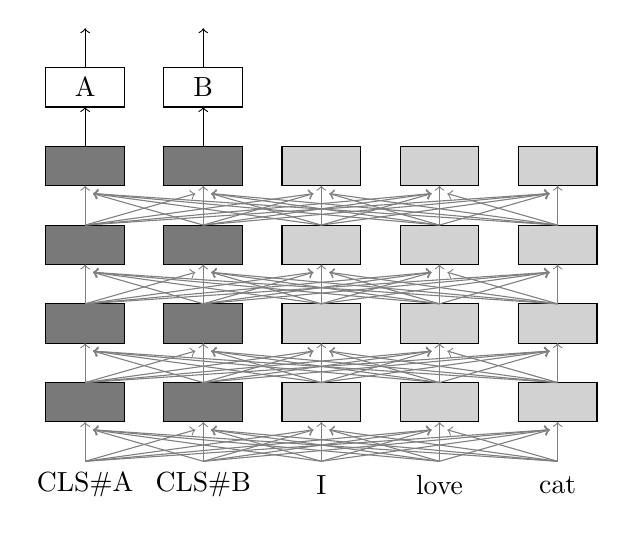
\begin{tikzpicture}
	\begin{scope}[fill opacity = .7 = .7]
	\draw [->, ] (-1.5, 5) -- (-1.5, 5.5);
	\draw [->, ] (-3, 5) -- (-3, 5.5);
	% 中间一列
	% modules
	\draw [fill=lightgray, draw = black] (-.5, 1) rectangle (.5, .5);
	\draw [fill=lightgray, draw = black] (-.5, 2) rectangle (.5, 1.5);
	\draw [fill=lightgray, draw = black] (-.5, 3) rectangle (.5, 2.5);
	\draw [fill=lightgray, draw = black] (-.5, 4) rectangle (.5, 3.5);
	% lines
	\draw [->, , gray ] (0, 0) -- (0, .5);
	\draw [->, , gray ] (0, 0) -- (-1.4, .4);
	\draw [->, , gray ] (0, 0) -- (1.4, .4);
	\draw [->, , gray ] (0, 0) -- (2.9, .4);
	\draw [->, , gray ] (0, 0) -- (-2.9, .4);
	
	\draw [->, , gray ] (0, 1) -- (0, 1.5);
	\draw [->, , gray ] (0, 1) -- (-1.4, 1.4);
	\draw [->, , gray ] (0, 1) -- (1.4, 1.4);
	\draw [->, , gray ] (0, 1) -- (2.9, 1.4);
	\draw [->, , gray ] (0, 1) -- (-2.9, 1.4);
	
	\draw [->, , gray ] (0, 2) -- (0, 2.5);
	\draw [->, , gray ] (0, 2) -- (-1.4, 2.4);
	\draw [->, , gray ] (0, 2) -- (1.4, 2.4);
	\draw [->, , gray ] (0, 2) -- (2.9, 2.4);
	\draw [->, , gray ] (0, 2) -- (-2.9, 2.4);
	
	\draw [->, , gray ] (0, 3) -- (0, 3.5);
	\draw [->, , gray ] (0, 3) -- (-1.4, 3.4);
	\draw [->, , gray ] (0, 3) -- (1.4, 3.4);
	\draw [->, , gray ] (0, 3) -- (2.9, 3.4);
	\draw [->, , gray ] (0, 3) -- (-2.9, 3.4);
	% 最左
	% modules
	\draw [fill=darkgray, draw = black] (-3.5, 1) rectangle (-2.5, .5);
	\draw [fill=darkgray, draw = black] (-3.5, 2) rectangle (-2.5, 1.5);
	\draw [fill=darkgray, draw = black] (-3.5, 3) rectangle (-2.5, 2.5);
	\draw [fill=darkgray, draw = black] (-3.5, 4) rectangle (-2.5, 3.5);
	\draw [draw = black] (-3.5, 5) rectangle (-2.5, 4.5);
	% lines
	\draw [->, , gray ] (-3, 0) -- (-3, .5);
	\draw [->, , gray ] (-3, 0) -- (-1.6, .4);
	\draw [->, , gray ] (-3, 0) -- (-.1, .4);
	\draw [->, , gray ] (-3, 0) -- (1.4, .4);
	\draw [->, , gray ] (-3, 0) -- (2.9, .4);
	
	\draw [->, , gray ] (-3, 1) -- (-3, 1.5);
	\draw [->, , gray ] (-3, 1) -- (-1.6, 1.4);
	\draw [->, , gray ] (-3, 1) -- (-.1, 1.4);
	\draw [->, , gray ] (-3, 1) -- (1.4, 1.4);
	\draw [->, , gray ] (-3, 1) -- (2.9, 1.4);
	
	\draw [->, , gray ] (-3, 2) -- (-3, 2.5);
	\draw [->, , gray ] (-3, 2) -- (-1.6, 2.4);
	\draw [->, , gray ] (-3, 2) -- (-.1, 2.4);
	\draw [->, , gray ] (-3, 2) -- (1.4, 2.4);
	\draw [->, , gray ] (-3, 2) -- (2.9, 2.4);
	
	\draw [->, , gray ] (-3, 3) -- (-3, 3.5);
	\draw [->, , gray ] (-3, 3) -- (-1.6, 3.4);
	\draw [->, , gray ] (-3, 3) -- (-.1, 3.4);
	\draw [->, , gray ] (-3, 3) -- (1.4, 3.4);
	\draw [->, , gray ] (-3, 3) -- (2.9, 3.4);
	
	\draw [->, ] (-3, 4) -- (-3, 4.5);
	
	% 左二
	% modules
	\draw [fill=darkgray, draw = black] (-2, 1) rectangle (-1, .5);
	\draw [fill=darkgray, draw = black] (-2, 2) rectangle (-1, 1.5);
	\draw [fill=darkgray, draw = black] (-2, 3) rectangle (-1, 2.5);
	\draw [fill=darkgray, draw = black] (-2, 4) rectangle (-1, 3.5);
	\draw [draw = black] (-2, 5) rectangle (-1, 4.5);
	% lines
	\draw [->, , gray ] (-1.5, 0) -- (-1.5, .5);
	\draw [->, , gray ] (-1.5, 0) -- (-.1, .4);
	\draw [->, , gray ] (-1.5, 0) -- (1.4, .4);
	\draw [->, , gray ] (-1.5, 0) -- (2.9, .4);
	\draw [->, , gray ] (-1.5, 0) -- (-2.9, .4);
	
	\draw [->, , gray ] (-1.5, 1) -- (-1.5, 1.5);
	\draw [->, , gray ] (-1.5, 1) -- (-.1, 1.4);
	\draw [->, , gray ] (-1.5, 1) -- (1.4, 1.4);
	\draw [->, , gray ] (-1.5, 1) -- (2.9, 1.4);
	\draw [->, , gray ] (-1.5, 1) -- (-2.9, 1.4);
	
	\draw [->, , gray ] (-1.5, 2) -- (-1.5, 2.5);
	\draw [->, , gray ] (-1.5, 2) -- (-.1, 2.4);
	\draw [->, , gray ] (-1.5, 2) -- (1.4, 2.4);
	\draw [->, , gray ] (-1.5, 2) -- (2.9, 2.4);
	\draw [->, , gray ] (-1.5, 2) -- (-2.9, 2.4);
	
	\draw [->, , gray ] (-1.5, 3) -- (-1.5, 3.5);
	\draw [->, , gray ] (-1.5, 3) -- (-.1, 3.4);
	\draw [->, , gray ] (-1.5, 3) -- (1.4, 3.4);
	\draw [->, , gray ] (-1.5, 3) -- (2.9, 3.4);
	\draw [->, , gray ] (-1.5, 3) -- (-2.9, 3.4);
	
	\draw [->, ] (-1.5, 4) -- (-1.5, 4.5);
	
	% 右2
	% modules
	\draw [fill=lightgray, draw = black] (1, 1) rectangle (2, .5);
	\draw [fill=lightgray, draw = black] (1, 2) rectangle (2, 1.5);
	\draw [fill=lightgray, draw = black] (1, 3) rectangle (2, 2.5);
	\draw [fill=lightgray, draw = black] (1, 4) rectangle (2, 3.5);
	% lines
	\draw [->, , gray ] (1.5, 0) -- (1.5, .5);
	\draw [->, , gray ] (1.5, 0) -- (-1.4, .4);
	\draw [->, , gray ] (1.5, 0) -- (.1, .4);
	\draw [->, , gray ] (1.5, 0) -- (2.9, .4);
	\draw [->, , gray ] (1.5, 0) -- (-2.9, .4);
	
	\draw [->, , gray ] (1.5, 1) -- (1.5, 1.5);
	\draw [->, , gray ] (1.5, 1) -- (-1.4, 1.4);
	\draw [->, , gray ] (1.5, 1) -- (.1, 1.4);
	\draw [->, , gray ] (1.5, 1) -- (2.9, 1.4);
	\draw [->, , gray ] (1.5, 1) -- (-2.9, 1.4);
	
	\draw [->, , gray ] (1.5, 2) -- (1.5, 2.5);
	\draw [->, , gray ] (1.5, 2) -- (-1.4, 2.4);
	\draw [->, , gray ] (1.5, 2) -- (.1, 2.4);
	\draw [->, , gray ] (1.5, 2) -- (2.9, 2.4);
	\draw [->, , gray ] (1.5, 2) -- (-2.9, 2.4);
	
	\draw [->, , gray ] (1.5, 3) -- (1.5, 3.5);
	\draw [->, , gray ] (1.5, 3) -- (-1.4, 3.4);
	\draw [->, , gray ] (1.5, 3) -- (.1, 3.4);
	\draw [->, , gray ] (1.5, 3) -- (2.9, 3.4);
	\draw [->, , gray ] (1.5, 3) -- (-2.9, 3.4);
	
	
	% 最右
	% modules
	\draw [fill=lightgray, draw = black] (2.5, 1) rectangle (3.5, .5);
	\draw [fill=lightgray, draw = black] (2.5, 2) rectangle (3.5, 1.5);
	\draw [fill=lightgray, draw = black] (2.5, 3) rectangle (3.5, 2.5);
	\draw [fill=lightgray, draw = black] (2.5, 4) rectangle (3.5, 3.5);
	% lines
	\draw [->, , gray ] (3, 0) -- (3, .5);
	\draw [->, , gray ] (3, 0) -- (-1.4, .4);
	\draw [->, , gray ] (3, 0) -- (.1, .4);
	\draw [->, , gray ] (3, 0) -- (1.6, .4);
	\draw [->, , gray ] (3, 0) -- (-2.9, .4);
	
	\draw [->, , gray ] (3, 1) -- (3, 1.5);
	\draw [->, , gray ] (3, 1) -- (-1.4, 1.4);
	\draw [->, , gray ] (3, 1) -- (.1, 1.4);
	\draw [->, , gray ] (3, 1) -- (1.6, 1.4);
	\draw [->, , gray ] (3, 1) -- (-2.9, 1.4);
	
	\draw [->, , gray ] (3, 2) -- (3, 2.5);
	\draw [->, , gray ] (3, 2) -- (-1.4, 2.4);
	\draw [->, , gray ] (3, 2) -- (.1, 2.4);
	\draw [->, , gray ] (3, 2) -- (1.6, 2.4);
	\draw [->, , gray ] (3, 2) -- (-2.9, 2.4);
	
	\draw [->, , gray ] (3, 3) -- (3, 3.5);
	\draw [->, , gray ] (3, 3) -- (-1.4, 3.4);
	\draw [->, , gray ] (3, 3) -- (.1, 3.4);
	\draw [->, , gray ] (3, 3) -- (1.6, 3.4);
	\draw [->, , gray] (3, 3) -- (-2.9, 3.4);
	
	\end{scope}
	
	% 输入句子
	\node at (-3, -.3) {CLS\#A};
	\node at (-1.5, -.3) {CLS\#B};
	\node at (0, -.3) {I};
	\node at (1.5, -.3) {love};
	\node at (3, -.3) {cat};
	
	\node at (-3, 4.75) {A};
	\node at (-1.5, 4.75) {B};
	\end{tikzpicture}
	\caption{L-E结构}
	\label{fig:l-e}
\end{figure}

在L-E结构输入时,为每一个任务并列地设置一个不同的\texttt{CLS}记号,因此可以看作是S-C结构的横向扩展,但L-E结构的任务特定模块被堆叠在该任务的\texttt{CLS}相对应的那一列。L-E结构允许任务在形成自己每一层的句子表示时窃听其他任务是如何抽象句子特征的。

\section{实现细节}
\label{sec:imp}

\subsection{训练过程}
为了避免可能出现的个别任务长时间不被选中的情况,本文采取的训练方式与一般的做法\footnote{可参考《神经网络与深度学习》第十章(\url{https://nndl.github.io})或相关文献\cite{Caruana1997}}稍有不同。下面的算法~\ref{alg:train}~给出了具体的训练算法。

\begin{algorithm}
	\caption{多任务联合训练过程}
	\label{alg:train}
	\begin{algorithmic}[1]
		\Require $M$~个任务的数据集~$\mathcal{D}_m, 1\le m \le M$;每个任务的批量大小~$K_m, 1\le m \le M$;最大迭代次数~$T$;学习率~$\alpha$.
		\Ensure 模型参数~$\theta$.
		\Function {TrainModel}{$\mathcal{D}_m$, $K_m$, $T$, $\alpha$}
		\State 初始化模型参数$\theta_0$
		\State 初始化任务列表$L$
		\For{$t=1 \cdots T$}
			\For{$m=1 \cdots M$}
				\State 将~$\mathcal{D}_m$~划分为~$c=N_m/K_m$~个小批量集合:
				$\mathcal{B}_m = \{ \mathcal{I}_{m,1},\cdots, \mathcal{I}_{m,c} \}$
			\EndFor
			\State $i = 1$
			\While {$|L|>0$}
			\State 打乱任务列表$L$顺序
			\For {\textbf{each} $m \in L$}
			\If {$\mathcal{I}_{m,i}$存在}
			\State 计算小批量样本$\mathcal{I}_{m,i}$上的损失$\mathcal{L}$
			\State 更新参数:$\theta_t = \theta_{t-1}-\alpha \cdot \nabla_\theta \mathcal{L}(\theta) $
			\Else 
			\State 将$m$从任务列表$L$中删除
			\EndIf
			\EndFor
			\State $i = i + 1$
			\EndWhile

		\EndFor
		\State \Return $\theta_T$
		\EndFunction
	\end{algorithmic}
\end{algorithm}

在多任务联合训练时,也存在一部分较为复杂的训练策略。例如,除了通过均匀采样的方式挑选任务外,还可以按数据集比例为不同任务分配被选中的概率\cite{sanh2018hierarchical};也可以预先定义任务采样策略\cite{DBLP:journals/tacl/KiperwasserB18};还可以采用不确定性来为不同任务的损失函数分配权重\cite{DBLP:conf/cvpr/KendallGC18}。

\subsection{超参数设定}
实验中使用的均为4层Transformer,模型维度为300,包含6个头,每个头为50维,前馈网络隐层维度为512维。使用Adam算法\cite{kingma2015adam}进行参数学习,初始学习率为5e-4,最多训练30个轮次。我们使用的小批量(mini-batch)大小为50. 

实验中采用的词向量为在840B词汇量的Common Crawl预料集上预训练的300维GloVe\cite{DBLP:conf/emnlp/PenningtonSM14}。为避免学习算法对GloVe进行过多的修改,我们为词嵌入层设置了更小的学习率:6e-4.

对于S-P结构,实现时在输出预测前叠加了一层多层感知机(MLP)以增强其效果,其余结构无此设置。前文提到的神经网络均基于PyTorch和fastNLP\footnote{fastNLP:\url{https://github.com/fastnlp/fastNLP}}实现,所有实验可在一张NVIDIA TITAN Xp上进行。
\chapter{实验}
\label{cha:exp}
本章介绍验证模型结构所进行的实验。首先,使用Transformer作为基线模型实验了单任务学习下的模型性能,接着使用相同的超参设定实验了~\ref{sec:mtl_tf}~节介绍的四种多任务Transformer的性能。具体地,在第~\ref{sec:task}~节介绍实验任务,在第~\ref{sec:ds}~节介绍数据集相关信息,在第~\ref{sec:results}~节介绍实验结果。最后,~\ref{sec:analysis}~节给出了实验分析。

\section{任务描述}
\label{sec:task}
我们在\emph{文本分类}(Text Classification)这一经典NLP任务上进行实验。事实上,很多NLP问题都可以归为文本分类的范畴,例如情感分析(Sentiment Analysis, SA)、自然语言推理(Natural Language Inference, NLI)等。在目前被广泛使用的多任务基准数据集GLUE\cite{DBLP:conf/emnlp/WangSMHLB18}中,所有任务都可以被归为文本分类任务。

文本分类即将一段归到某个特定的预先定义的类别。待分类的文本通常是一个句子(如情感分析)或一个句子对(如自然语言推理)。需要注意的是,这里的一个句子并不一定是常规意义上以一个句号为结束标识符的一句话,也有可能包含多句话。文本分类任务在现实生活中也有着广泛的应用,如自动分析产品评价、微博情感分析、文档标签分类等等。

文本分类任务需要模型能够抽取出易于分类的句子表示,然而不同领域中通常需要关注不同的特征,例如在食物类的评论文本中模型应当更加关注“好吃”、“美味”等词,而在电影评论文本中应当更加关注“好看”、“烂片”等词语。同时,不同领域的文本分类任务常常也需要某些通用的特征,如“很棒”、“优秀”等词在所有与主观倾向有关的分类任务中都是应当被关注的。而事实上,在某个特定的领域内,文本数据量常常是有限的,这种情况下单任务学习通常难以取得很好的效果,可以通过多任务学习来利用其他领域的相关知识帮助分类。

\section{数据集}
\label{sec:ds}
我们的基线单任务模型以及多任务模型在16个文本分类数据集上进行了对比实验,其中的前14个数据集来自亚马逊的产品评论\footnote{\url{https://www.cs.jhu.edu/˜mdredze/datasets/ sentiment/}},但是来自各自不同的领域,如图书、电子、光盘等。该部分数据由Blitzer等人\cite{DBLP:conf/acl/BlitzerDP07}收集而成,其余两个数据集IMDB\cite{DBLP:conf/acl/MaasDPHNP11}和MR\cite{DBLP:conf/acl/PangL05}则来自电影评论。每个数据集包含约2000个样本,其中70\%划分为训练集,10\%划分为验证集,20\%划分为测试集。数据集的具体统计信息见表~\ref{tb:dataset}。

\begin{table}[htb]
	\centering
	\caption{数据集统计数据}
	\begin{tabular}{ccccccc}
		\toprule[2pt]
		数据集&训练集大小&验证集大小&测试集大小&类别数&平均长度&词表大小\\
		\midrule[1pt]
		Books& 1400& 200& 400& 2& 159& 19K\\
		Elec& 1398& 200& 400& 2& 101& 11K\\
		DVD& 1400& 200& 400& 2& 173& 20K\\
		Kitchen& 1400& 200& 400& 2& 89& 9K\\
		Apparel& 1400& 200& 400& 2& 57& 7K\\
		Camera& 1397& 200& 400& 2& 130& 9K\\
		Health& 1400& 200& 400& 2& 81& 9K\\
		Music& 1400& 200& 400& 2& 136& 17K\\
		Toys& 1400& 200& 400& 2& 90& 10K\\
		Video& 1400& 200& 400& 2& 156& 17K\\
		Baby& 1300& 200& 400& 2& 104& 8K\\
		Mag& 1370& 200& 400& 2& 117& 11K\\
		Soft& 1315& 200& 400& 2& 129& 11K\\
		Sports& 1400& 200& 400& 2& 94& 10K\\
		IMDB& 1400& 200& 400& 2& 269& 25K\\
		MR& 1400& 200& 400& 2& 21& 7K\\
		\bottomrule[2pt]
	\end{tabular}
	\label{tb:dataset}
\end{table}

\section{实验结果}
\label{sec:results}
实验结果如表~\ref{tb:results}~所示,我们的四个多任务模型在十六个文本分类任务上均超过了单任务训练的表现,验证了多任务学习在Transformer上的有效性。其中,L-I结构在四种多任务架构中表现最好,S-P结构表现最差。L-I结构和L-E结构取得的较好结果表明,在每一层都形成任务特定表示的做法相比在网络的顶层获取特征更为合理。同时,注意到S-C结构也能达到较好的准确率,这也肯定了之前被广泛使用的硬共享模式的效果,但随着任务之间差异性的增大,我们有理由认为L-I和L-E的共享架构相比传统架构将表现出更大的优越性。

\begin{table}[htb]
	\centering
	\caption{模型在测试集上的分类准确率}
	\begin{tabular}{c|cccccc}
		\toprule[2pt]
		\multirow{2}*{数据集}&\multirow{2}*{单任务}&\multicolumn{4}{c}{多任务}\\
		\cline{3-6}
		&&S-P结构& S-C结构& L-I结构& L-E结构\\
		\midrule[1pt]
		Books& 83.50& 82.50& 84.00& 85.00& 84.50\\
		Elec& 79.50& 82.50& 83.50& 84.75& 85.75\\
		DVD& 82.75& 84.50& 85.50& 85.75& 85.75\\
		Kitchen& 79.50& 83.50& 85.00& 89.00& 87.75\\
		Apparel& 82.75& 85.50& 86.75& 86.00& 85.75\\
		Camera& 81.75& 84.25& 85.00& 87.00& 89.00\\
		Health& 86.00 & 85.50& 87.50& 88.00& 86.75\\
		Music& 76.50& 83.00& 83.00& 82.75& 81.50\\
		Toys& 80.00& 84.75& 86.25& 88.25& 86.50\\
		Video& 84.75& 81.25& 85.50& 86.50& 84.25\\
		Baby& 81.00 &87.75& 85.50& 87.25& 87.50\\
		Mag& 89.00& 85.00& 91.00& 89.75& 89.25\\
		Soft& 86.50& 86.00& 88.75& 86.50& 87.75\\
		Sports& 80.25& 84.25& 83.75& 86.00& 85.50\\
		IMDB& 80.75& 84.75& 85.00& 84.50& 84.50\\
		MR& 75.25& 76.00& 75.75& 78.00& 76.50\\
		\rowcolor{lightgray}
		AVG.& 81.86& 83.81& 85.11& \textbf{85.94}& 85.53\\
		\bottomrule[2pt]
	\end{tabular}
	\label{tb:results}
\end{table}

在实践中,神经网络的层数通常是一个比较重要的超参数,模型性能有时会由于层数的不同而产生较大差异。之前的实验中使用的模型均为4层Transformer,为探究多任务Transformer结构对网络层数的敏感性,我们实验了四种结构在不同层数下的平均分类准确率,结果如图~\ref{fig:layer_dis}~所示。

可见,在各个层数设定中,逐层共享结构(L-I结构和L-E结构)均优于传统的硬共享结构(S-P结构和S-C结构),且L-I结构在三种设定中都取得了最优准确率,这一实验结果证明了模型的鲁棒性。

\begin{figure}[htb]
\centering
\begin{tikzpicture}
\begin{axis}[
	xlabel={层数},
	ylabel={准确率},
	legend style={
		cells={anchor=east},
		legend pos=outer north east,
	}
]

\addplot coordinates{
	(2, 0.8547)
	(4, 0.8594)
	(6, 0.8523)
};

\addplot coordinates{
	(2, 0.8539)
	(4, 0.8553)
	(6, 0.8500)
};

\addplot [mark=x]coordinates {
	(2, 0.8451)
	(4, 0.8381)
	(6, 0.8167)
};

\addplot coordinates{
	(2, 0.8484)
	(4, 0.8511)
	(6, 0.8478)
};
\legend{L-I结构,L-E结构,S-P结构,S-C结构}
\end{axis}
\end{tikzpicture}
\caption{网络层数对测试集准确率的影响}
\label{fig:layer_dis}
\end{figure}

\section{实验分析}
\label{sec:analysis}

\begin{figure}[htb]
\centering
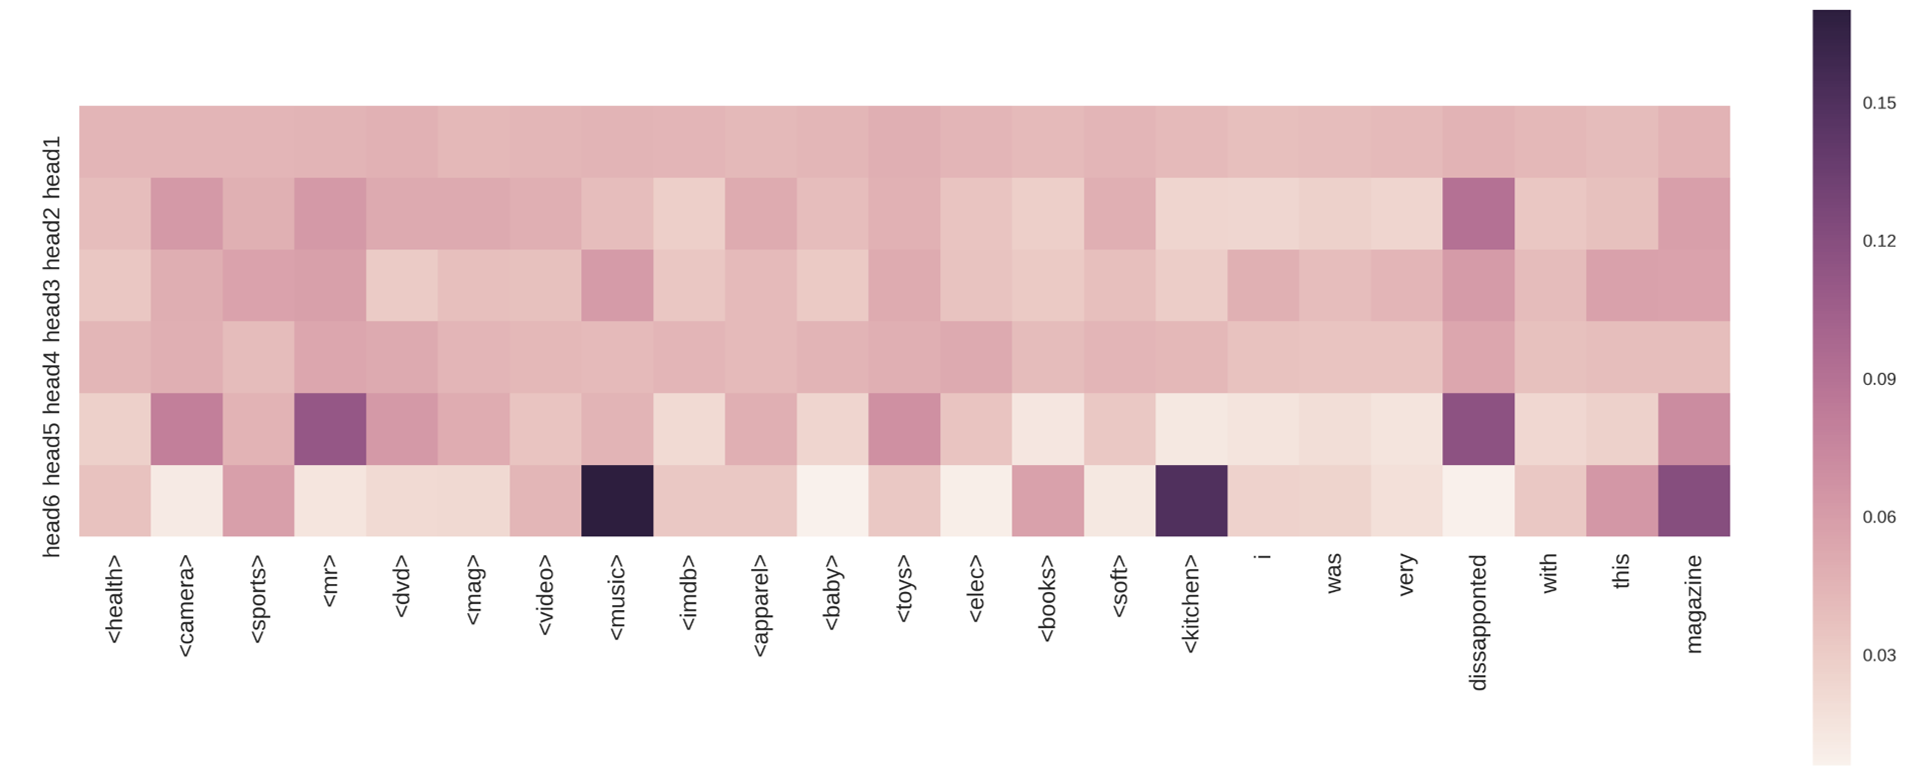
\includegraphics[scale=0.4]{L-E-attn.png}
\caption{L-E结构注意力可视化}
\label{fig:l-e-attn}
\end{figure}
\chapter{总结与展望}
\label{cha:conclusions}
本章首先对已有工作以及本文的研究内容进行了总结,概括了本文工作的贡献,也指出了不足。随后,对多任务自然语言处理的研究前景进行了展望,给出了未来的的研究方向。

\section{工作总结}
学习文本的分布式表示一直以来都是基于神经网络的自然语言处理模型的关键问题,文本数据特征表示的好坏直接决定着模型的性能。在数据量或计算资源有限的情况下,传统的单任务方法常常难以学习到泛化的特征表示。因此,多任务学习作为一种学习泛化表示的手段被广泛应用到各类神经网络中。

多任务学习的本质在于参数共享,如何设计有效的共享模式一直是多任务学习的研究重点。一方面,多任务学习中的很多共享模式是模型无关的,可以不加修改地应用在各类模型上,如硬共享模式。另一方面,对于特定的网络和任务常常又需要设计特定的共享模式。

近年来,很多研究人员在卷积神经网络和循环神经网络上应用多任务学习,在自然语言处理、计算机视觉、语音识别等应用领域都取得了成功。然而,目前还很少有工作探索多任务学习在Transformer上的应用模式和效果。本文旨在一定程度上填补这一空缺,验证了多任务学习在Transformer结构上的有效性,并针对Transformer结构特点提出了两种新型的共享模式:L-I共享模式和L-E共享模式,在多个文本分类任务上相比传统的硬共享模式取得了更高的准确率。本文的实验结果表明,在神经网络的每一层都提取任务特定表示具有

然而,本文提出的多任务学习模型架构也具有一定的局限性,只能适用于句子级别的任务,如文本分类任务,难以应用于序列标注任务中。如何为序列标注任务设计有效的多任务Transformer结构仍是需要解决的问题。

\section{未来展望}
目前主流的单任务学习方法常常使得神经网络模型受限于单一任务甚至数据集,在某个数据集上表现良好的模型可能在另一个数据集上表现很差。通过设置合适的训练任务,增大训练数据量可以得到具备强大泛化表示能力的可迁移模型,能够为很多NLP任务带来性能提升,这类方法的典型代表就是BERT。由于其带来的强大的性能提升和通用性,BERT在NLP社区获得了巨大反响,也引发了很多研究者的思考:是否能够训练单一模型来处理几乎所有的NLP任务?

但是近期的相关实验也表明,BERT在语义任务以及需要任务特定语法知识的任务上表现欠佳,对实体和指代现象的处理还不够好\cite{47786}\cite{liu2019linguistic},这说明,BERT在某些情况下也并非如此“通用”。如何赋予预训练模型更多知识呢?

近期,百度对BERT的训练任务进行了改进,提出了基于中文的预训练模型ERNIE,它具备了更多的实体知识。但其并未在根本上解决BERT面临的局限性。

造成这一局限性的一个关键原因在于,用来训练BERT的任务——语言模型和预测下一句话——并不能对所有NLP任务都带来很大提升。事实上,可能不存在某个单一预训练任务在所有目标任务下都非常有效。在这一背景下,一个很自然的想法便是利用多任务学习方法来训练。

事实上,迁移学习和多任务学习都是通过参数共享的方式来起作用。BERT采用的模型结构便是Transformer,因而BERT的成功也证明了Transformer强大的知识存储能力和可迁移性,这为多任务Transformer的有效性提供了保障。在BERT基础上,进一步使用多任务训练的方法已经被证明是有效的\cite{liu2019multi}。我相信,随着对多任务Transformer结构的探索,越来越多的任务可以被同时训练,相应的,也会有越来越多的任务知识可以共存于单一模型中。



%%%%%%%%%%%%%%%
%% 论文后置部分
%%%%%%%%%%%%%%%
\backmatter

%% 插图索引
% \listoffigures
%% 表格索引
% \listoftables

%% 致谢
\addcontentsline{toc}{chapter}{\bfseries{致谢}}

\begin{acknowledgments}

四载匆匆,倏忽而至,终于要毕业了。

我还清楚地记得那段穿着军装、踢着正步、烈日永远不会缺席的时光,记得敲下第一行\texttt{Hello World}时的懵懂,也还记得和队友们一起通宵做数模的疲惫,更记得无数个平凡的日子里坐在教室里一起听课的同学们和站在讲台上的教授们……一切仿佛就在昨日,如今却要离开这里了。

回首这段岁月,我只觉得幸运。何其幸运,能遇到这么多学识渊博、兢兢业业的老师;何其幸运,能遇到这么多优秀又谦虚的同学们。借此机会,我想向你们致以真挚的感谢。

首先,我想感谢本文的指导老师,也即将是我博士阶段的导师:邱锡鹏老师和黄萱菁老师。他们提供的悉心指导和实验环境为我毕业设计的顺利完成提供了保障。在几个月的相处中,邱老师的学术品味、研究热情和为人方式都让我受益匪浅,我相信我也将度过同样充实愉快的博士生涯。

然后,我要感谢本科阶段给予我巨大帮助的老师们和同学们。感谢陈慧婵老师和郭艳艳老师,他们为我打下了扎实的数理基础;感谢张淑平老师、张立勇老师和顾新老师,让我掌握了必要的专业知识;感谢周水生老师,在我的数模和科研上提供了大量指导。感谢一路同行的同学们,王磊、余天焕、徐之浩、班浩等等,你们一直是我成长路上的榜样;还要感谢陪伴我四年的室友,王敏锐、王许丞和冯尧,感谢你们一直以来的包容与帮助。

最后,我要感谢我的家人。感谢我的父母,在我的求学路上面临的每一次选择,你们都给予了最大的鼓励与信任,没有你们一如既往的支持,也不会有现在的我;还要感谢我的女朋友曲雪纯,遇到你是我本科阶段最大的收获之一。你们一直,也将永远是我最强大的后盾!

\begin{flushright}
	\emph{孙天祥}\\
	二零一九年五月于西电
\end{flushright}

\end{acknowledgments}


\cleardoublepage
% 参考文献
\addcontentsline{toc}{chapter}{\bfseries{参考文献}}
\bibliographystyle{gbt7714-2005}
\bibliography{refs}

\end{document}
